\chapter{Results}
\section{Implementation of Randomness in the Logistic Map}
% \begin{figure}[!h]
% \caption[Lyapunov exponent in the random logistic map]{The
%   Lyapunov exponent for the random logistic map, where $x_0=0.6$ for $r \in
%   [0,4]$. For $\lambda>0$, the system may be chaotic, and for $\lambda
%   <0$, the system is stable. The number of exponents computed over
%   [0,4] was $N_\lambda=10,000$.}\label{fig:detloglyap1}
% 	\begin{center}
% 		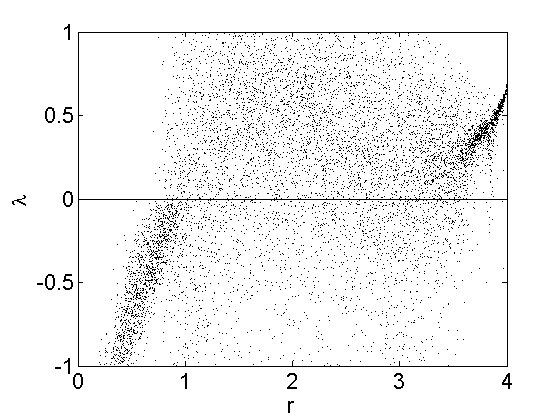
\includegraphics[scale=0.65]{figs/rlog_lyap_all.png}
% 	\end{center}
% \end{figure} 

\begin{figure}[!h]
\caption[Lyapunov exponent in the random logistic map compared to the
deterministic map]{The Lyapunov exponent for the deterministic
  logistic map (top left) is compared
  to the Lyapunov exponent of the random logistic map for $L \in \{0.05,0.1,0.5,0.7,0.9\}$, where $x_0=0.7$ for $r \in [3,4]$. The number of exponents computed over
  [3,4] was $N_\lambda=10,000$. Plots are read left to right, and top
  to bottom. }\label{fig:rloglyap2}
\centering
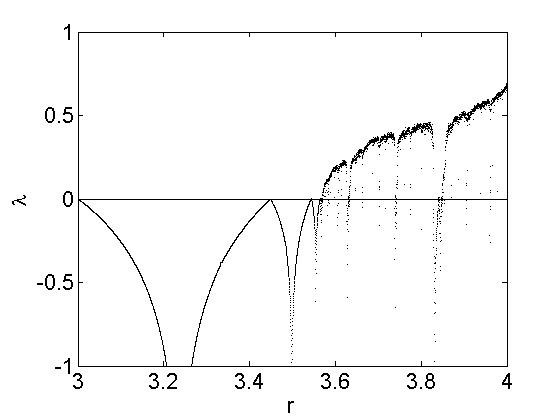
\includegraphics[width=.5\textwidth]{figs/det_log_lyap.png}\hfill
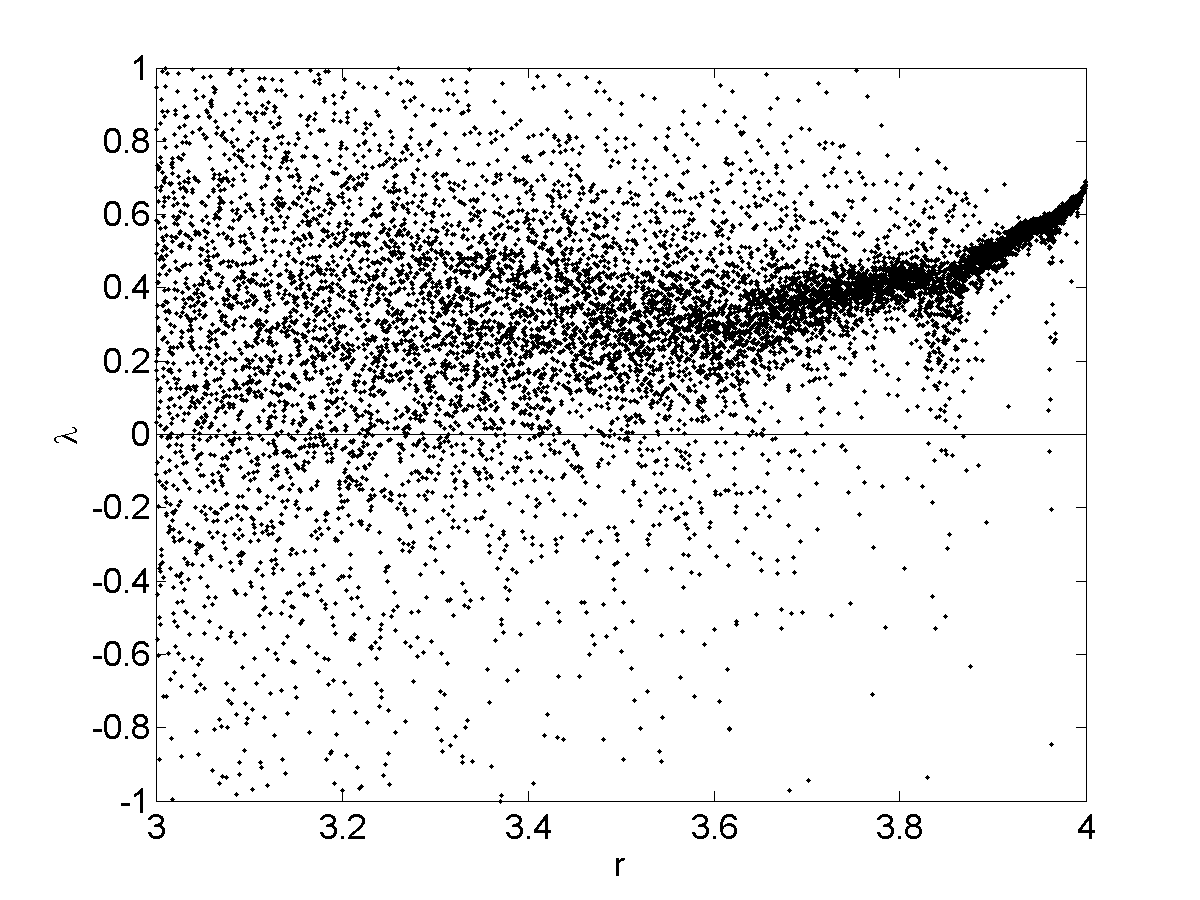
\includegraphics[width=.5\textwidth]{figs/rlog_lyap_L_005.png}\\
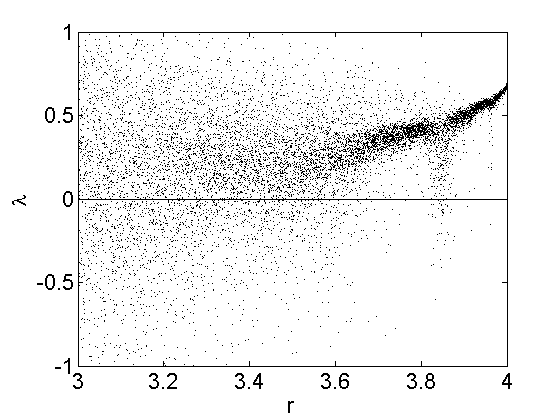
\includegraphics[width=.5\textwidth]{figs/rlog_lyap_L01_zoom.png}\hfill
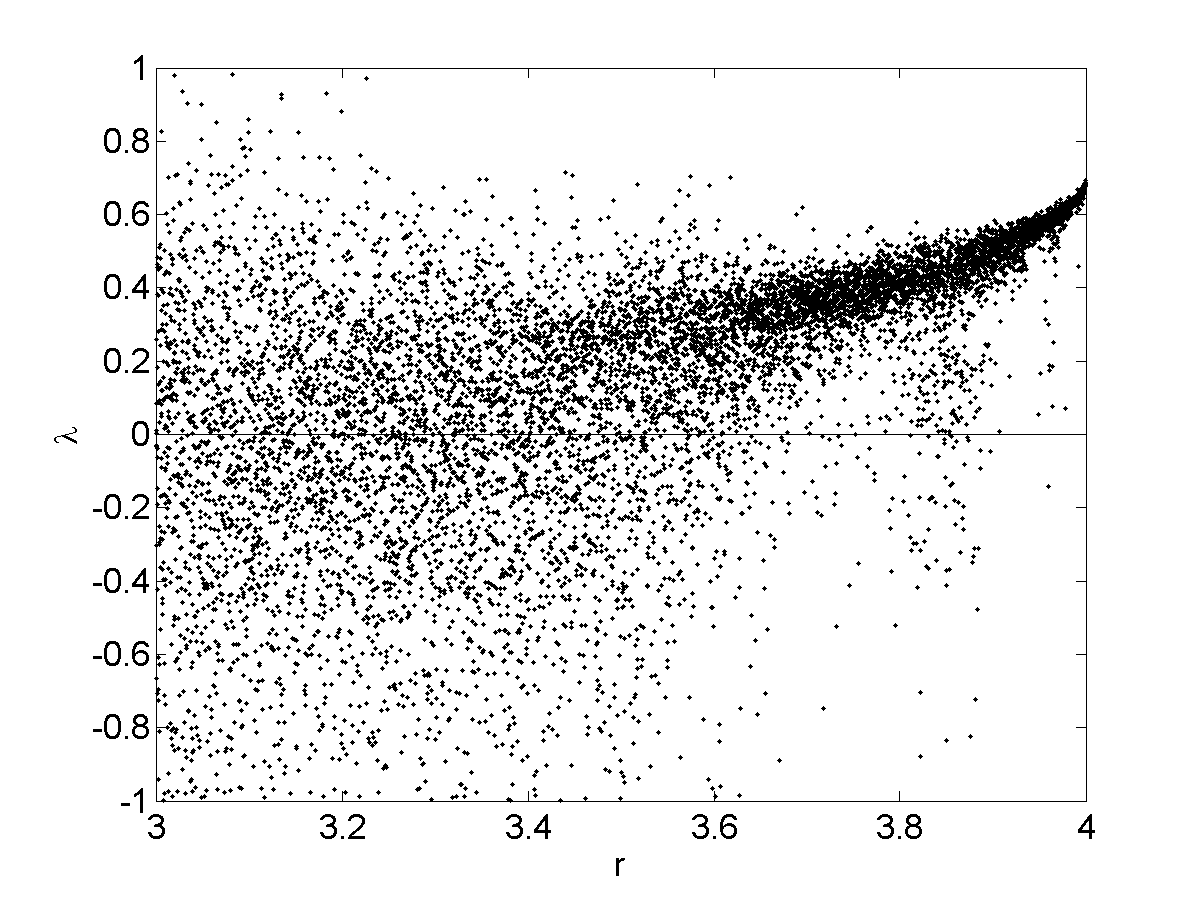
\includegraphics[width=.5\textwidth]{figs/rlog_lyap_L_05.png}\\
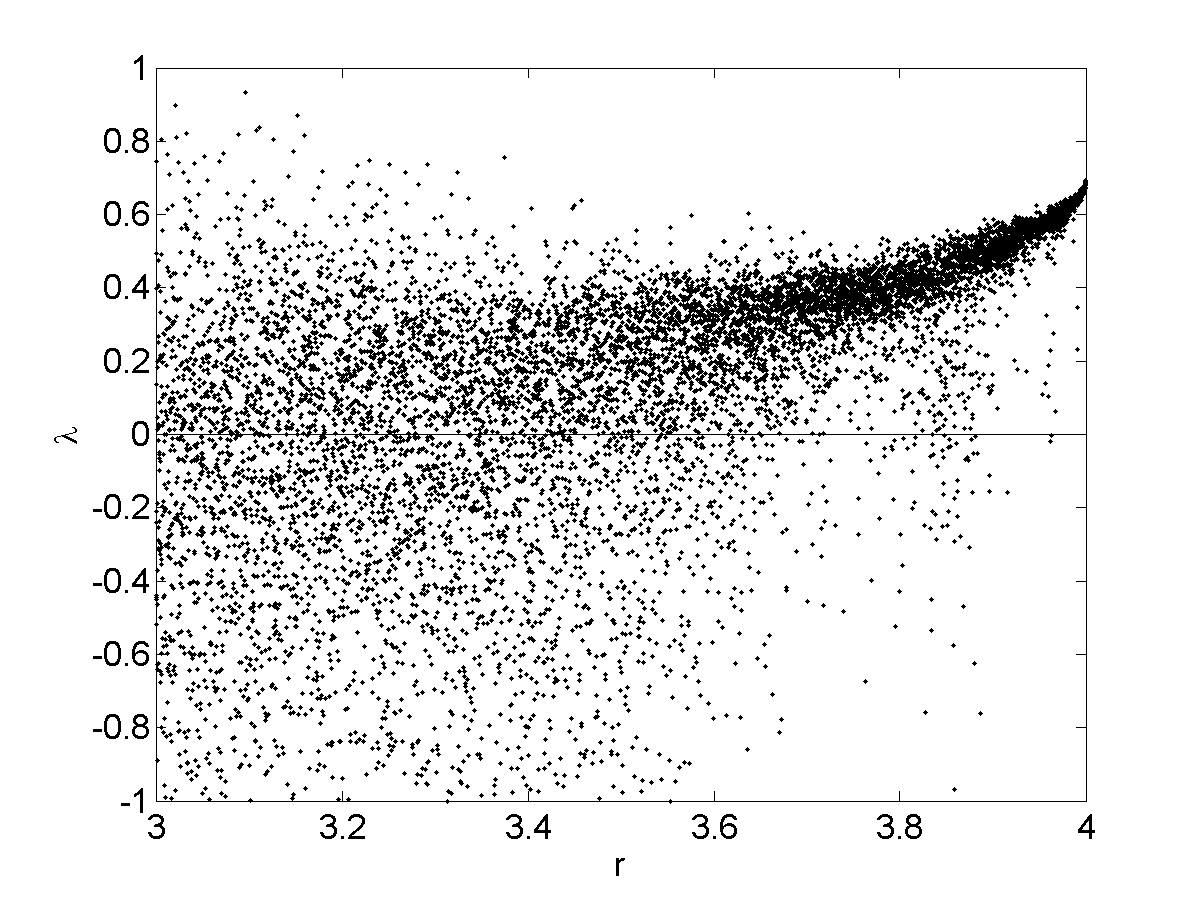
\includegraphics[width=.5\textwidth]{figs/rlog_lyap_L_07.png}\hfill
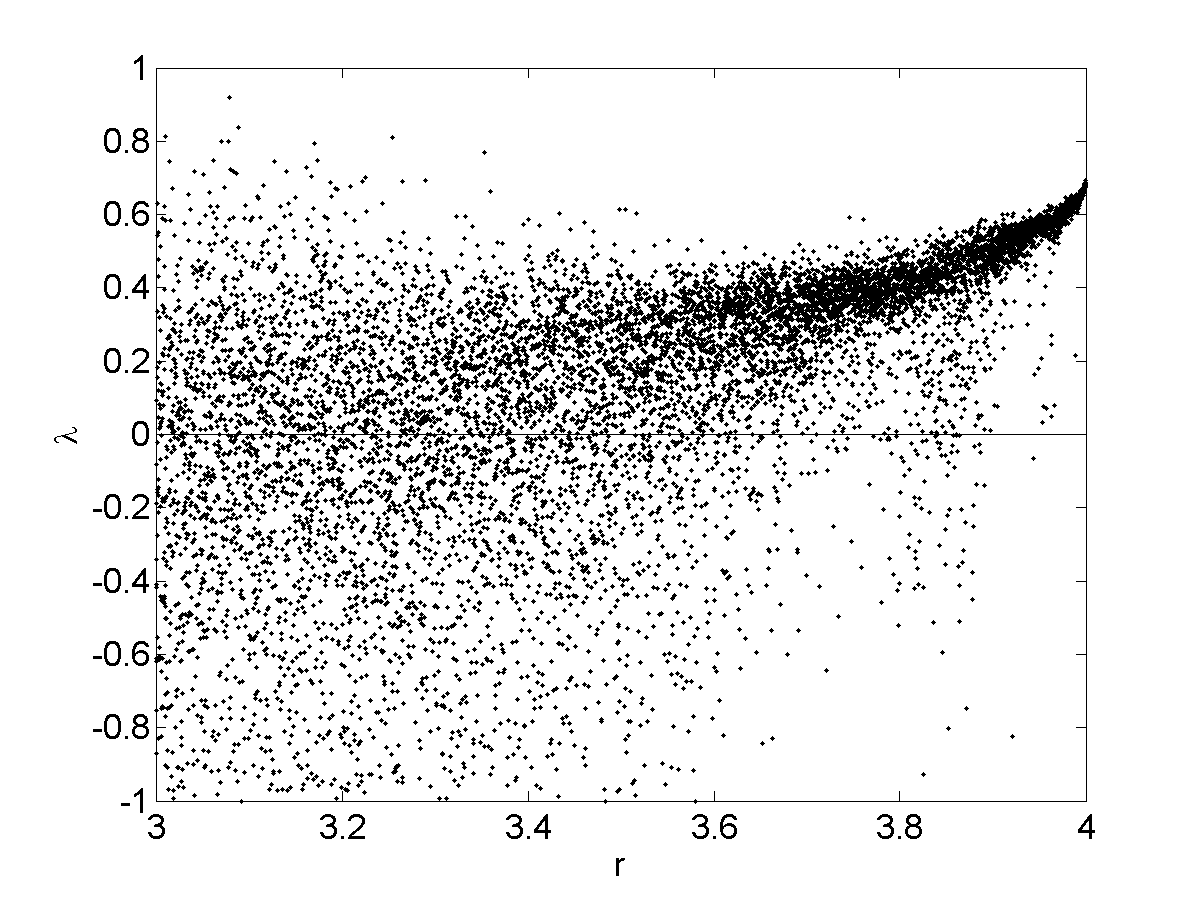
\includegraphics[width=.5\textwidth]{figs/rlog_lyap_L_09.png}\\
\end{figure}

\begin{figure}[H]\linespread{1}
\caption[Average number of order $p$ orbits for the random circle
map]{Average number of order $p$ orbits for the random circle
map, where $r =3.2$,$L=0.1$,$N=100$, and $\sigma = 0.0061$. Results from 2000
simulations of these parameters are plotted.}
	\begin{center}
          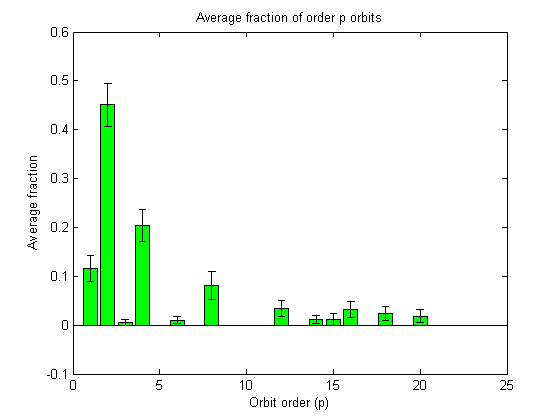
\includegraphics[scale=0.7]{figs/rlog_hist_r32_L01.png}
	\end{center}
\end{figure}

\begin{figure}[H]\linespread{1}
\caption[Random logistic map bifurcation diagram, low resolution]{A
  low-resolution bifurcation diagram of the random
logistic map, where $r \in [0,4]$, $\Delta r = 0.009$, $N=100$, the
number of initial conditions $N_{x_0}=100$, and $L=0.1$. Results from 45,000 simulations are plotted. The colorbar to the right
of the graph demonstrates the period order and corresponding color of
the orbit. Periodicity up to period order 52 was checked.}
	\begin{center}
          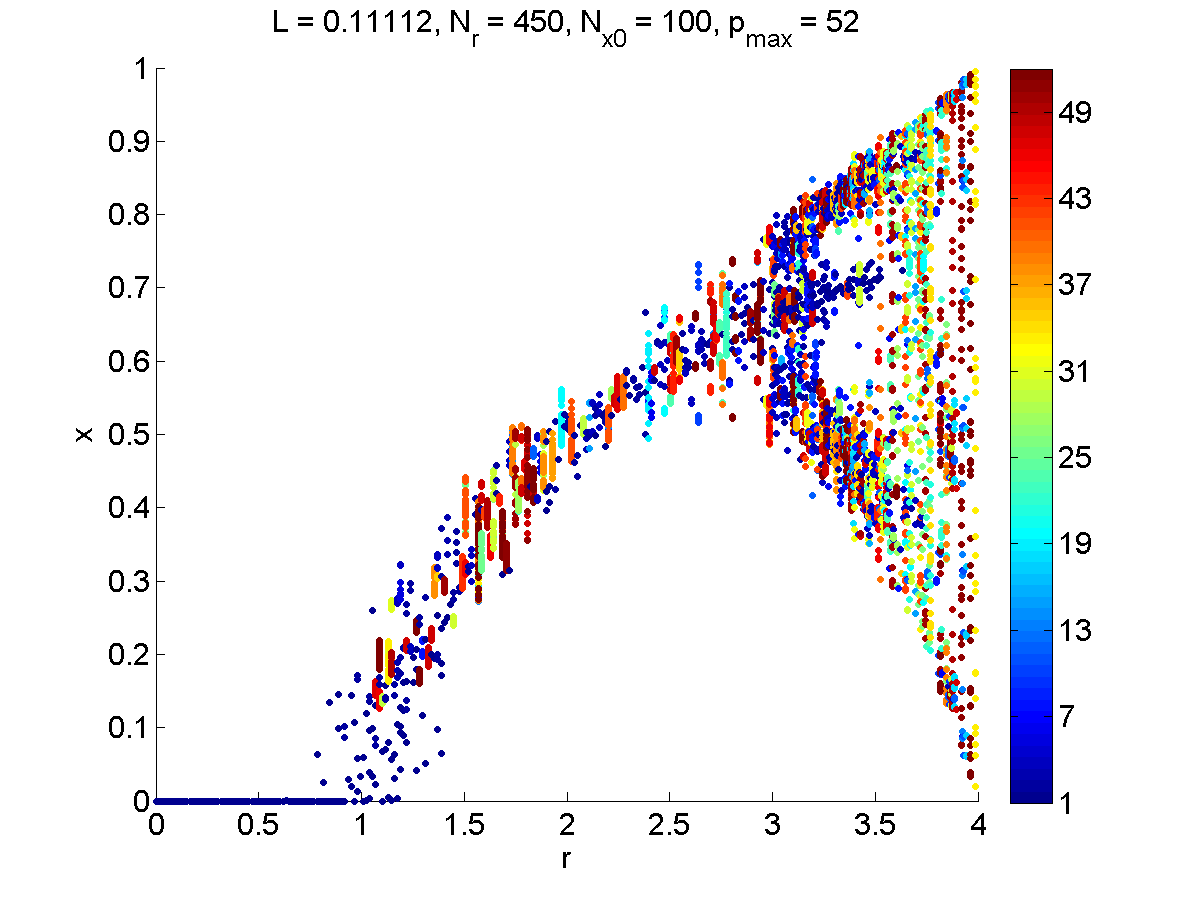
\includegraphics[scale=0.6]{figs/rlog_bif_L_01_low.png}
	\end{center}
\end{figure}


\begin{figure}[H]\linespread{1}
\caption[Bifurcation diagram of the random logistic map, high resolution]{Bifurcation diagram of the random
logistic map, where $r \in [0,4]$, $\Delta r = 0.002$, $N=100$, the
number of initial conditions $N_{x_0}=1000$, and $L\in
\{0.1,0.2,0.4,0.6,0.8,0.9\}$. Plots are read left to right, and top to
bottom. Results from 1.8 million simulations are plotted. The colorbar to the right
of the graph demonstrates the period order ($p\leq 256$) and corresponding color of
the orbit.}\label{fig:rlogbif}
	\begin{center}
		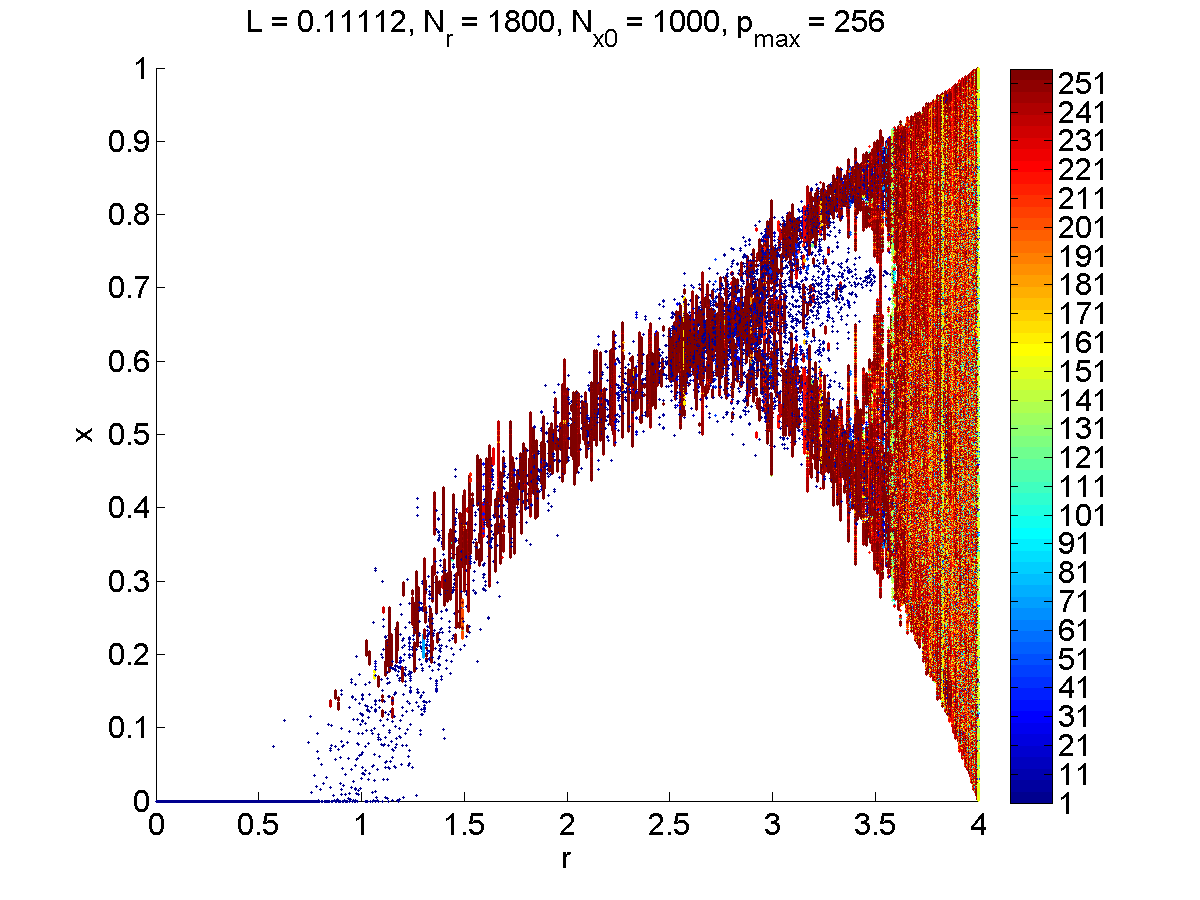
\includegraphics[width=.5\textwidth]{figs/rlog_bif_L_01.png}\hfill
		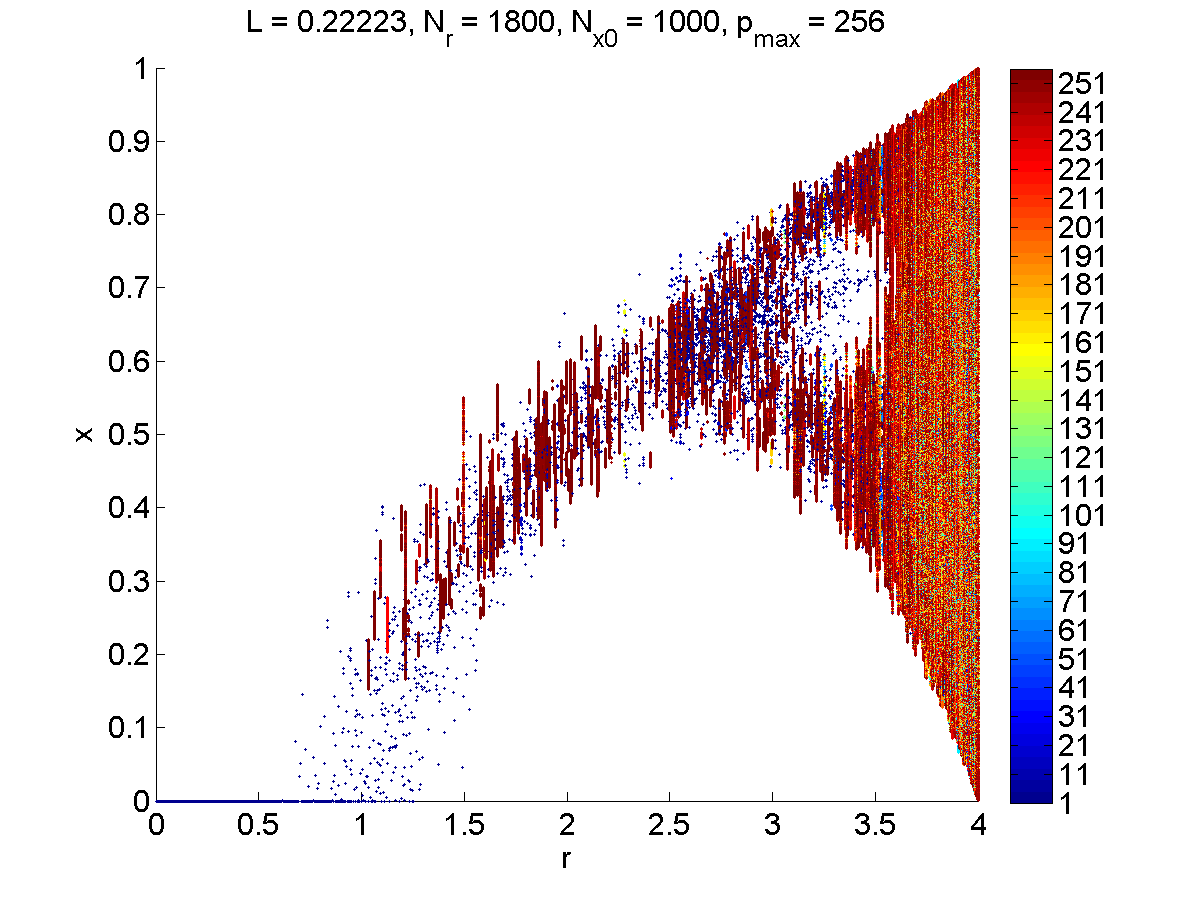
\includegraphics[width=.5\textwidth]{figs/rlog_bif_L_02.png}\\
		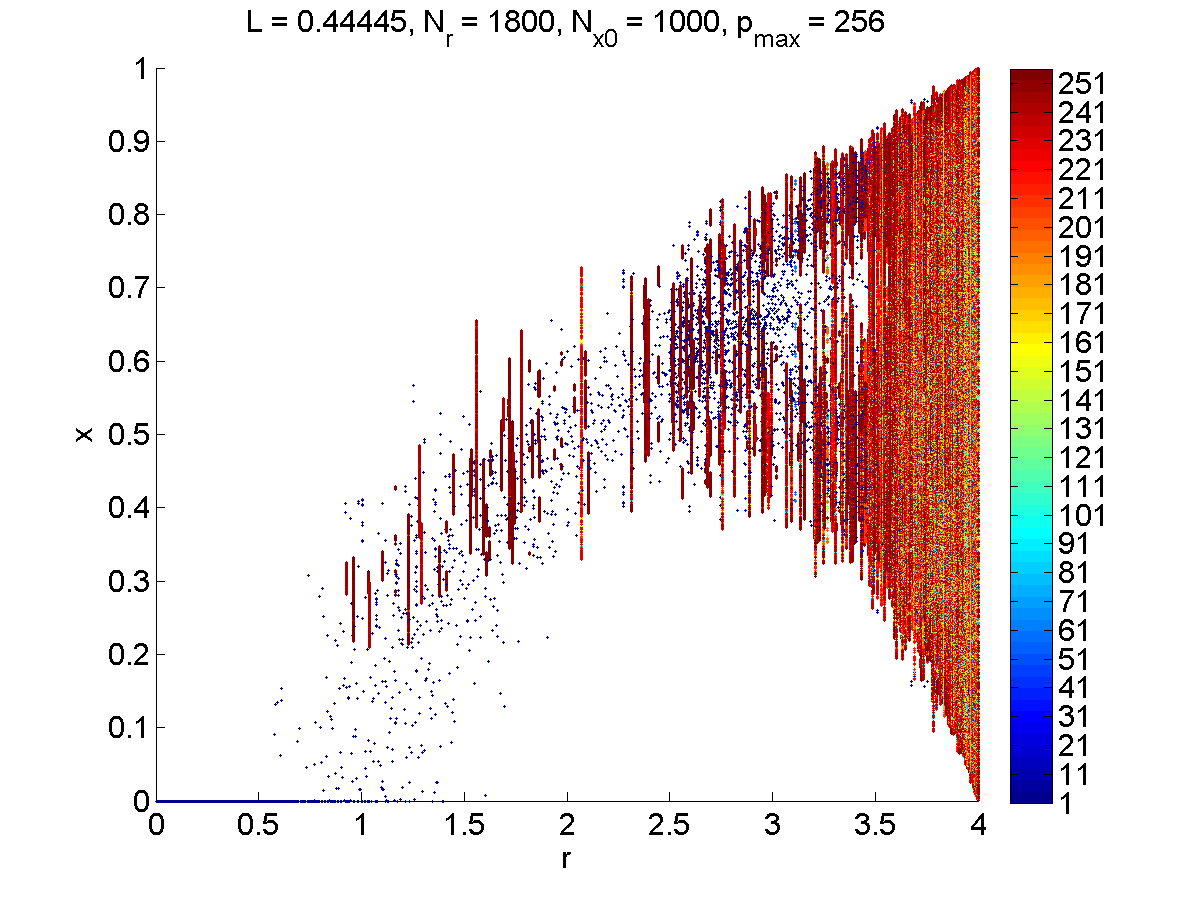
\includegraphics[width=.5\textwidth]{figs/rlog_bif_L_04.png}\hfill
		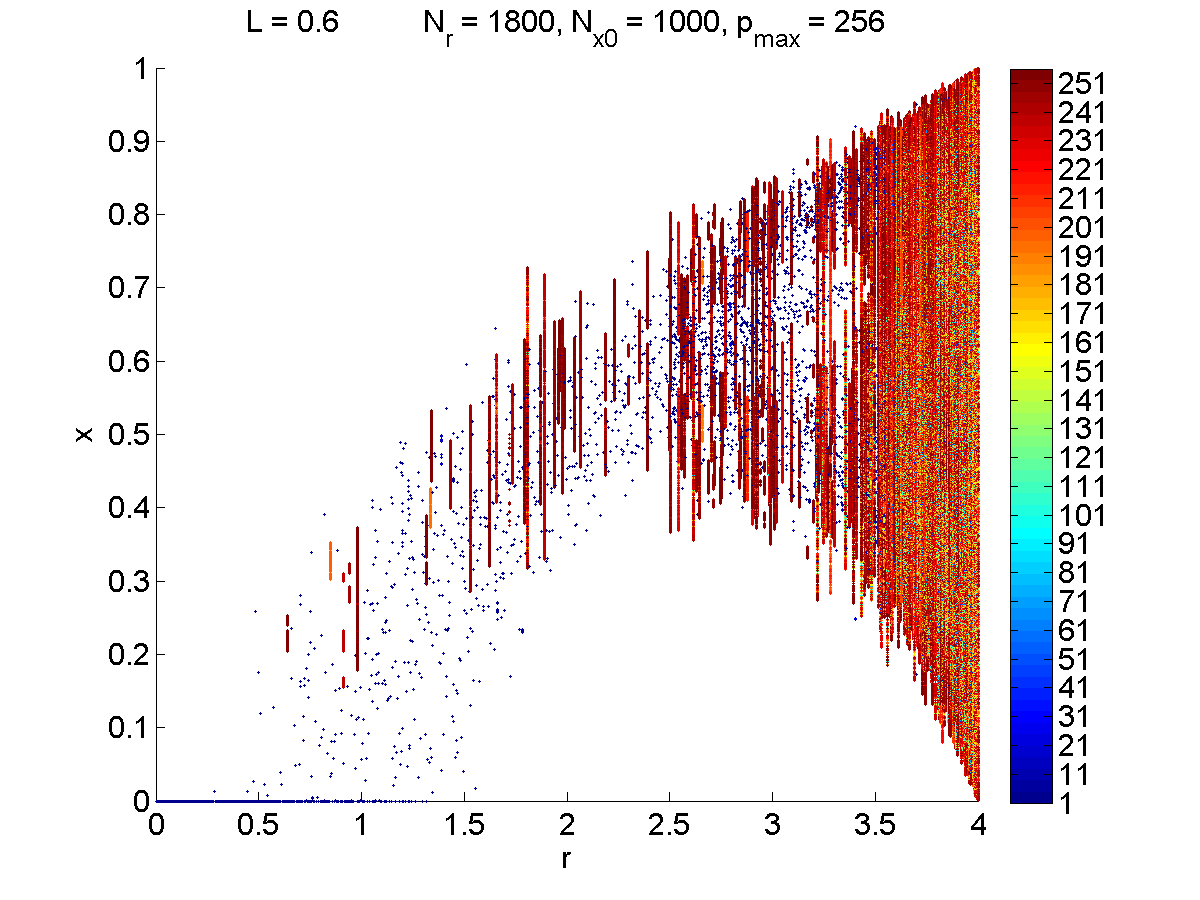
\includegraphics[width=.5\textwidth]{figs/rlog_bif_L_06.png}\\
		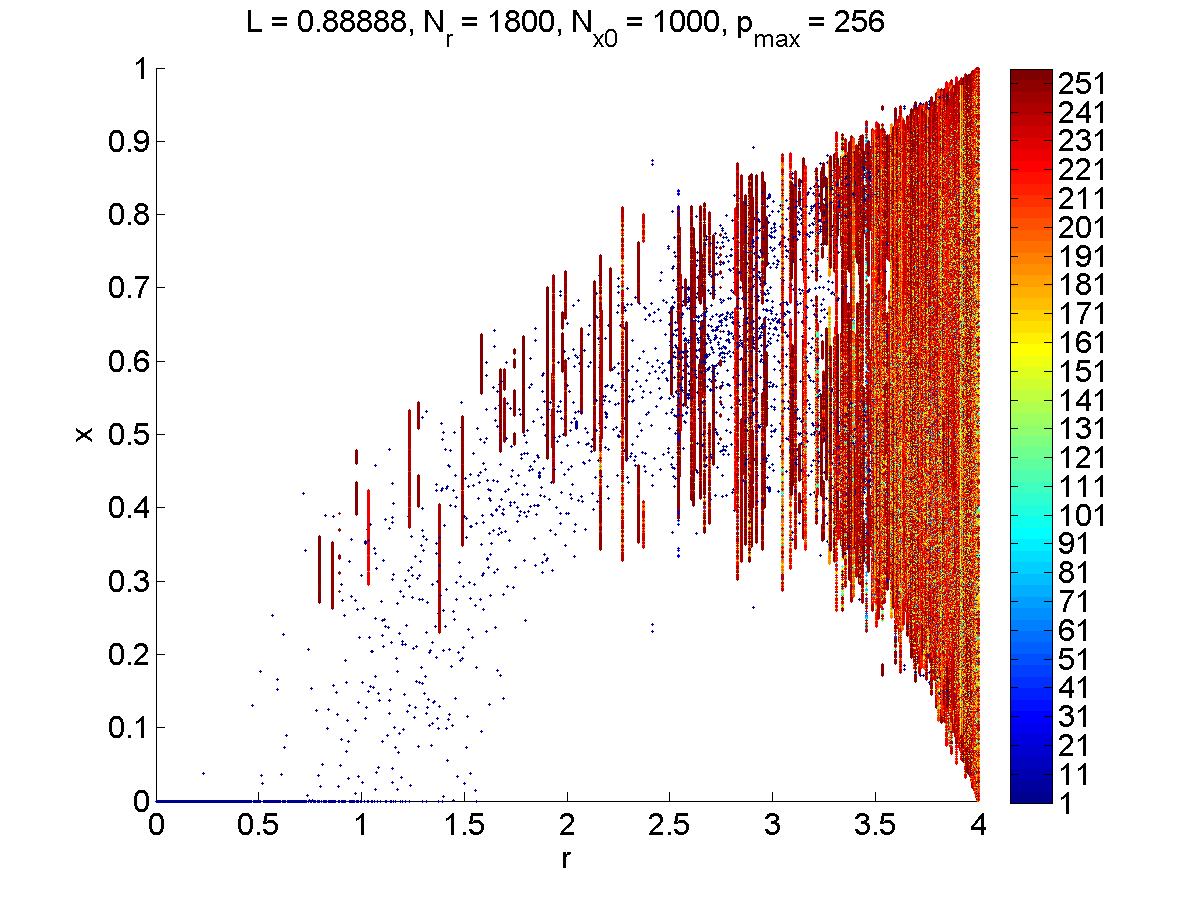
\includegraphics[width=.5\textwidth]{figs/rlog_bif_L_08.png}\hfill
		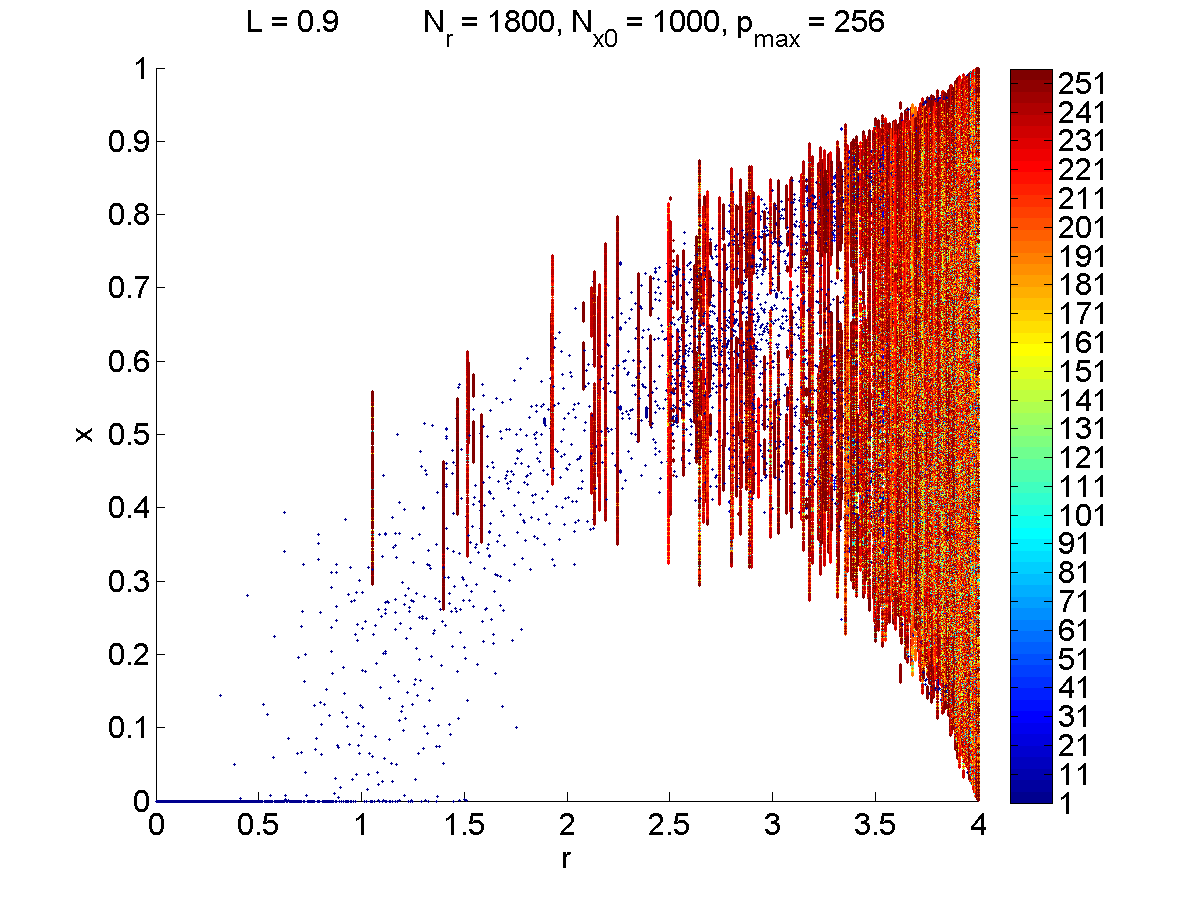
\includegraphics[width=.5\textwidth]{figs/rlog_bif_L_09.png}\\
	\end{center}
\end{figure}

\begin{figure}[H]\linespread{1}
\caption[Bifurcation diagram of the random logistic map, zoomed
in]{A zoomed in view of Figure~\ref{fig:rlogbif}, where $r \in
  [3,4]$, $\Delta r = 0.001$, $N=100$, the number of initial
  conditions $N_{x_0}=1000$, and $L\in \{0.1,0.2,0.4,0.6,0.8,0.9\}$.}
	\begin{center}
		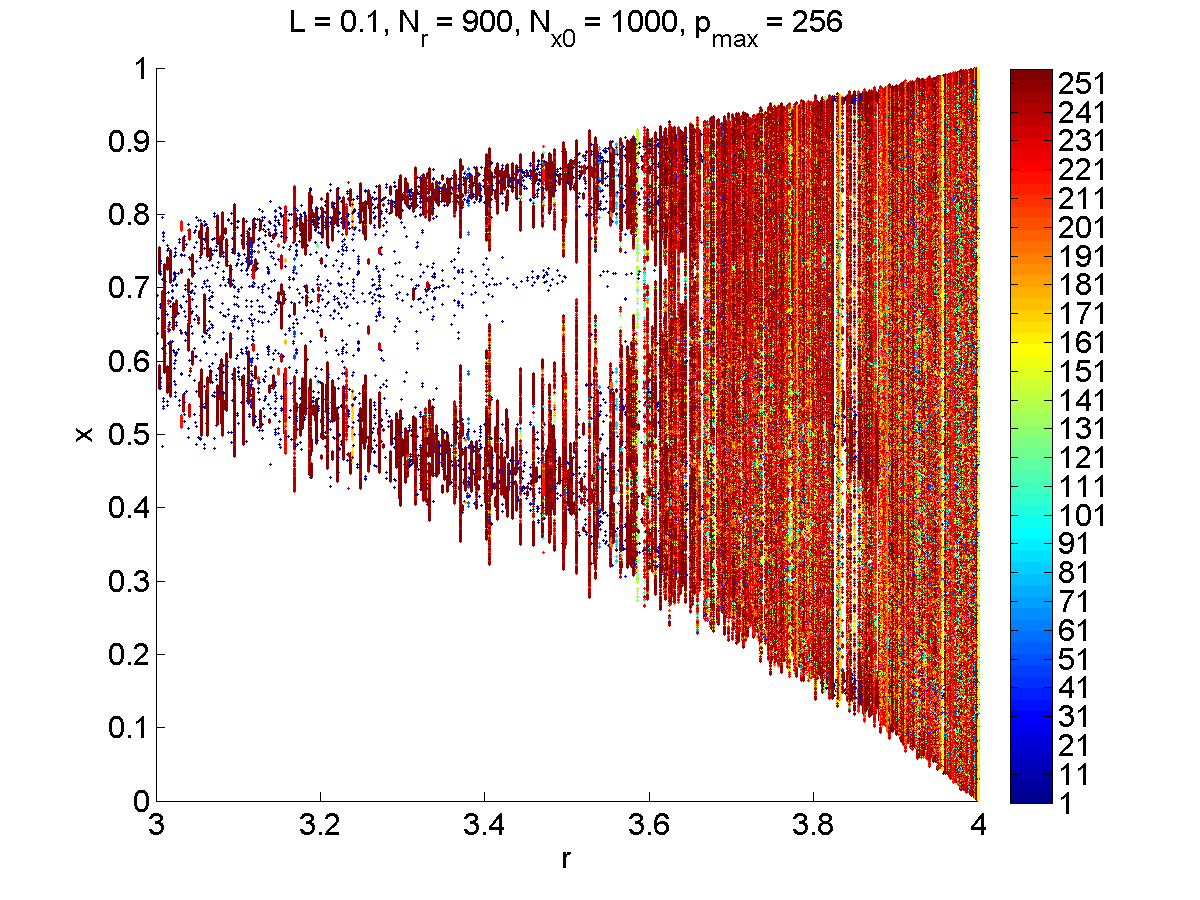
\includegraphics[width=.5\textwidth]{figs/rlog_bif_zoom_L_01.png}\hfill
		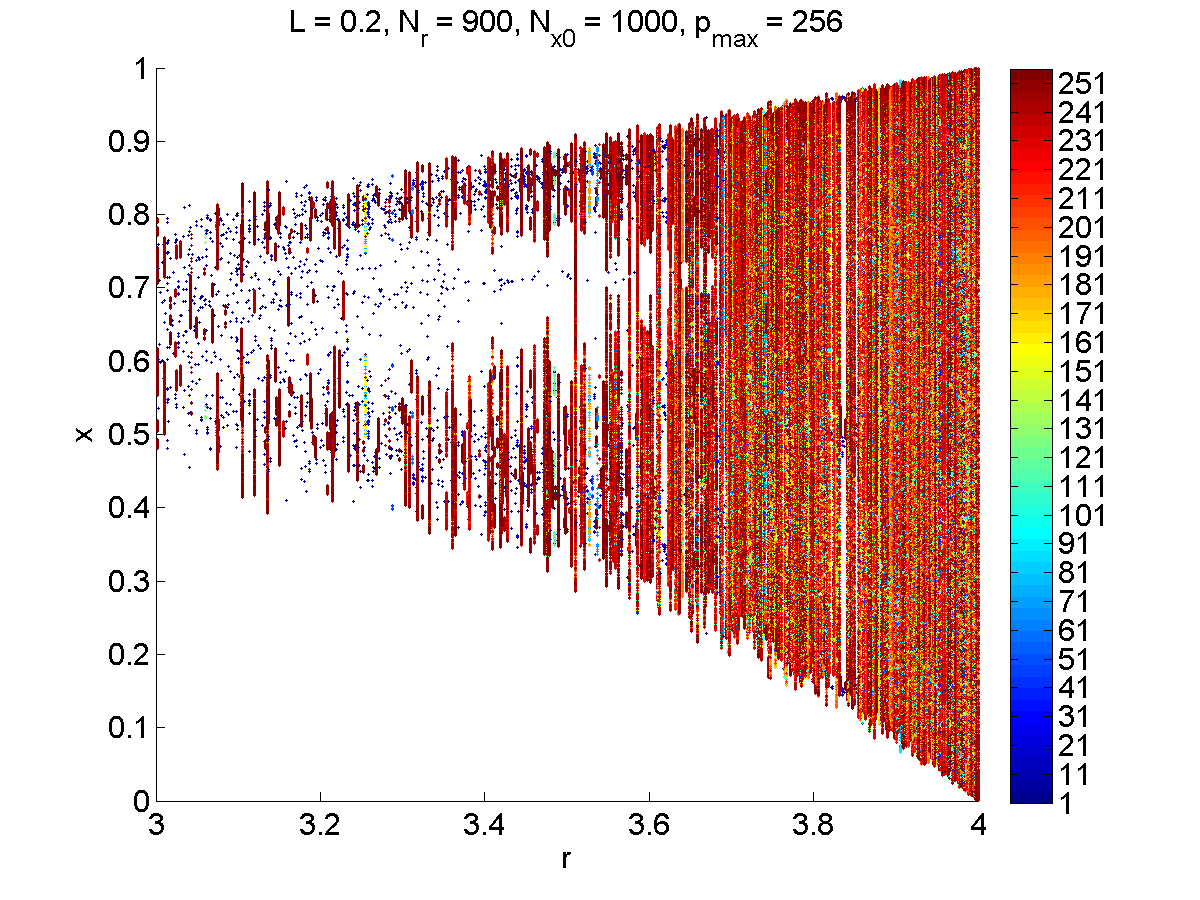
\includegraphics[width=.5\textwidth]{figs/rlog_bif_zoom_L_02.png}\\
		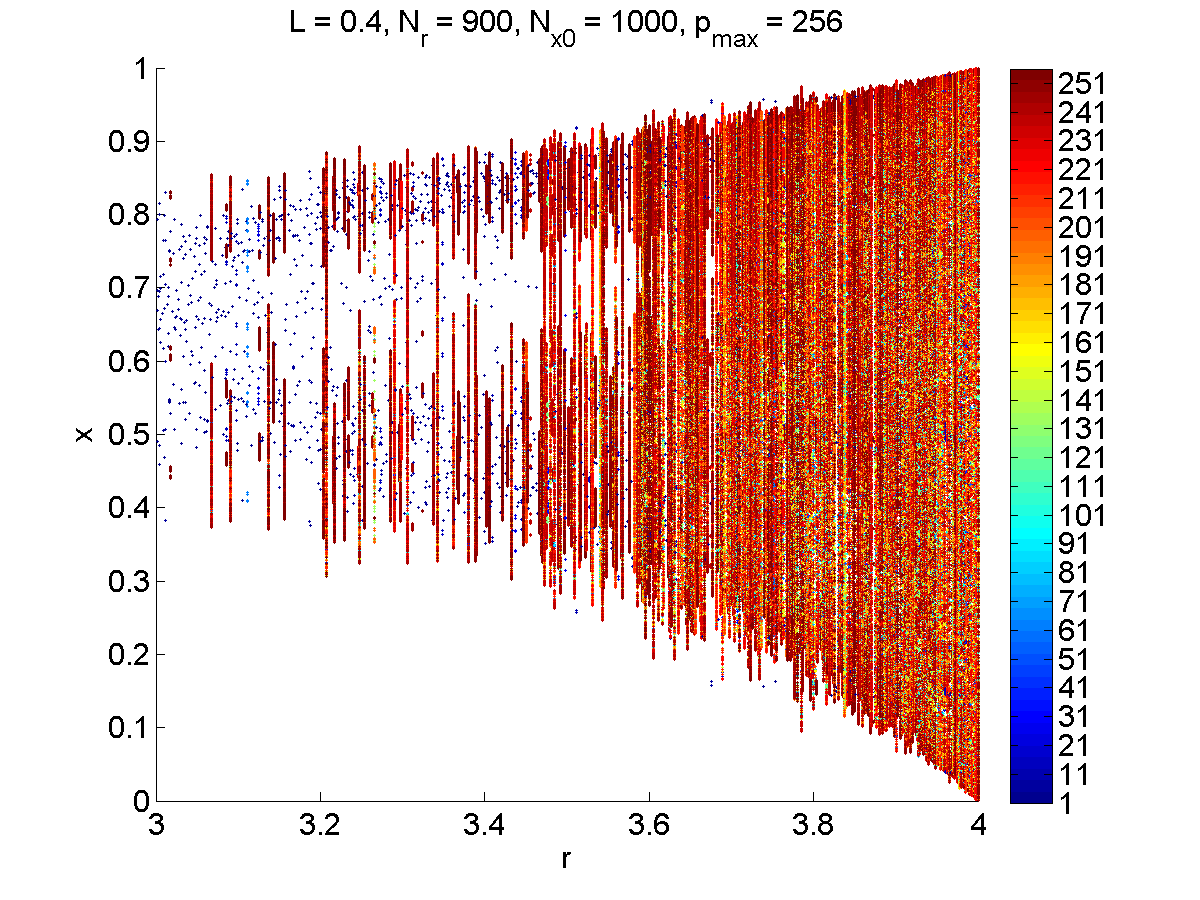
\includegraphics[width=.5\textwidth]{figs/rlog_bif_zoom_L_04.png}\hfill
		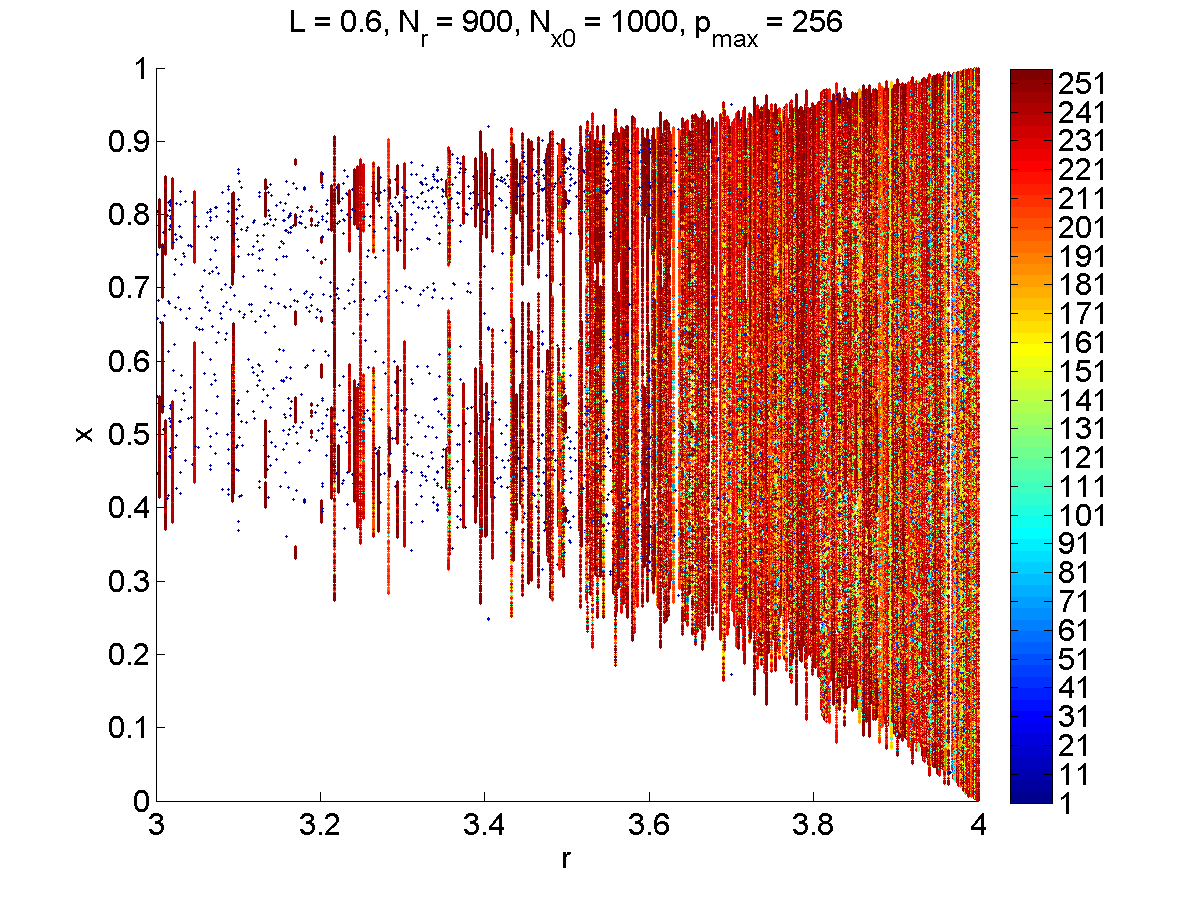
\includegraphics[width=.5\textwidth]{figs/rlog_bif_zoom_L_06.png}\\
		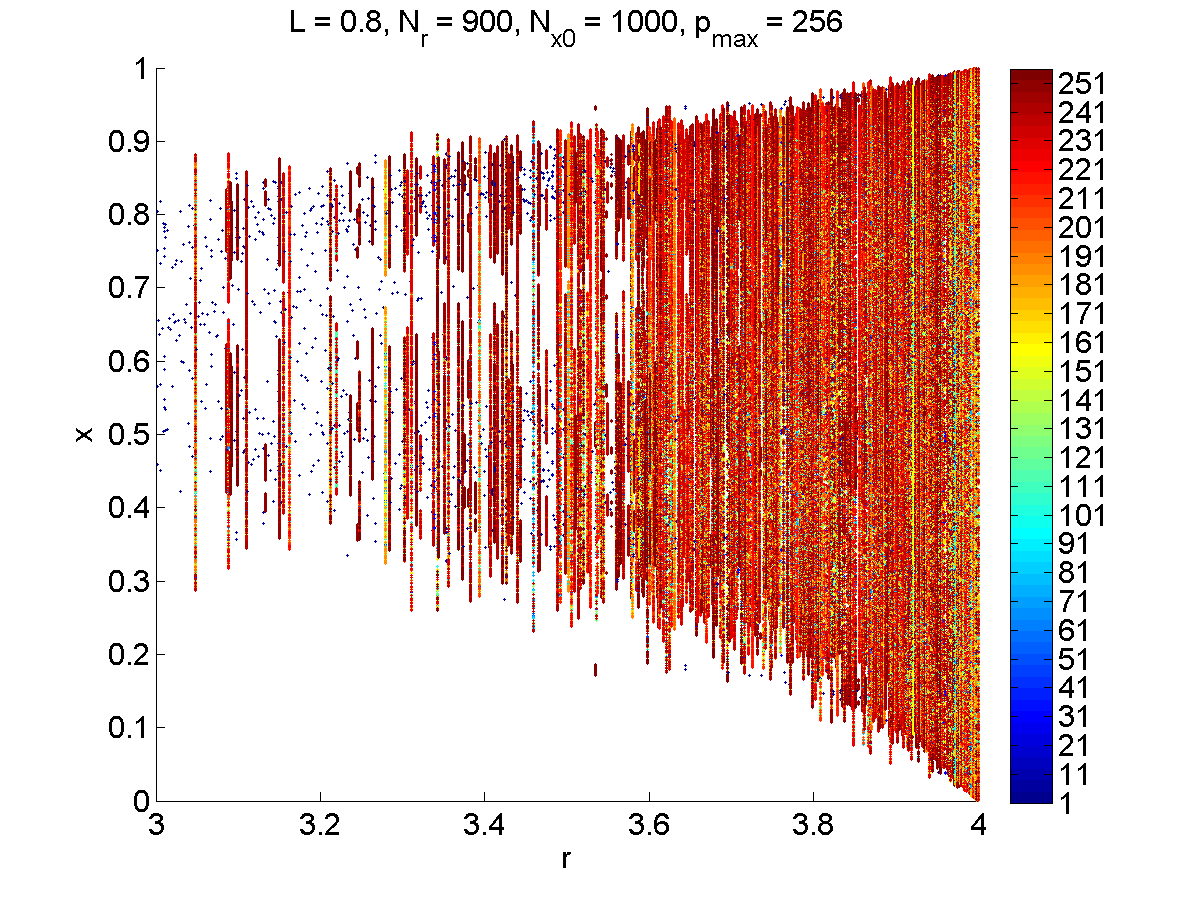
\includegraphics[width=.5\textwidth]{figs/rlog_bif_zoom_L_08.png}\hfill
		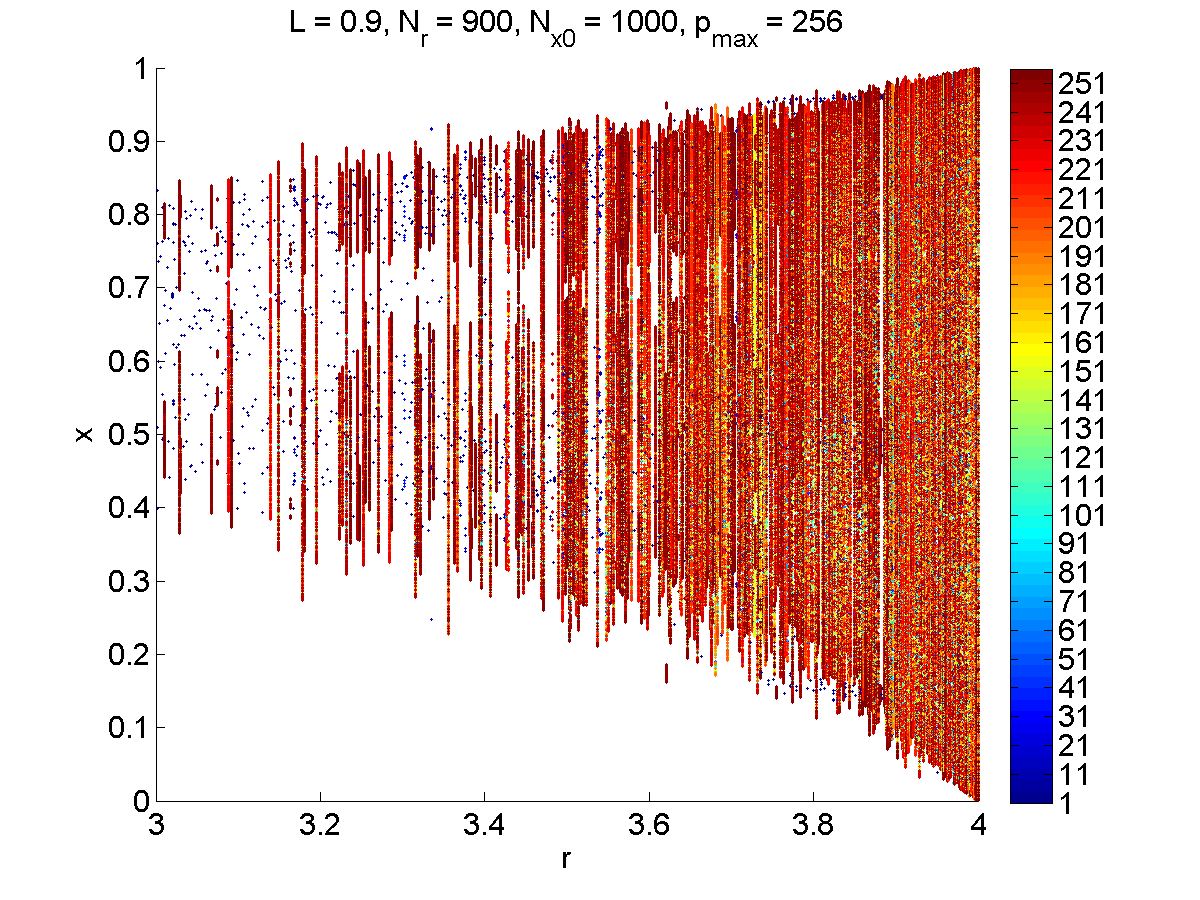
\includegraphics[width=.5\textwidth]{figs/rlog_bif_zoom_L_09.png}\\
	\end{center}
\end{figure}

\section{Implementation of Randomness in the Circle Map}
\subsection{Uniform Distribution}
\begin{figure}[H]\linespread{1}
\caption[Average number of order $p$ orbits for the random circle
map]{Average number of order $p$ periodic orbits for the random circle
map, where $L=0.1$, $\omega =0.1$, $\alpha = 10^{-5}$ and $k=1$. Results from 1000
simulations of these parameters are plotted.}
	\begin{center}
		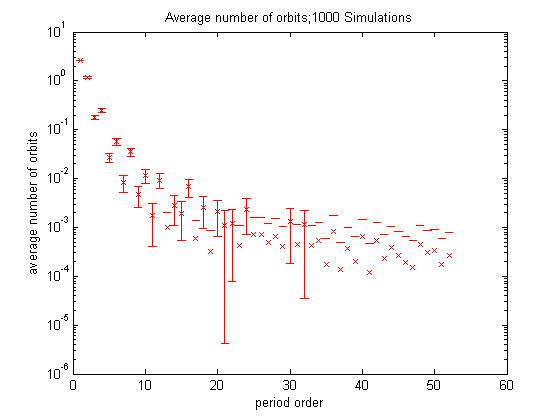
\includegraphics[scale=0.7]{figs/rcirc_avg_num_1000_sim_logscale.png}
	\end{center}
\end{figure}

\begin{figure}[H]\linespread{1}
\caption[Bifurcation diagram of the random
circle map]{Bifurcation diagram of the random
circle map for $L=0.1$, $\omega \in [0,1]$, $\Delta \omega = 0.001$,$\alpha = 10^{-5}$
and $k=1$. Results from 100 simulations of these parameters are
plotted. Blue: period 1, red:
period 2, cyan: period 3, magenta: period 4, green: period 5, black:
period $p > 5$.} 
	\begin{center}
		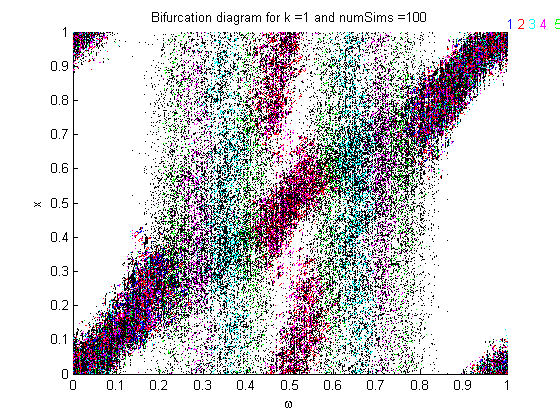
\includegraphics[scale=0.7]{figs/rcirc_bif_L01_k1.png}
	\end{center}
\end{figure}

\begin{figure}[H]\linespread{1}
\caption[The devil's staircase for the random circle map]{The devil's
  staircase for $k=1$,$\alpha = 10^{-5}$ and $L = 0.1,0.5$. For small $L$
  (leftmost graph), the noise is more pronounced than for large $L$
  (rightmost graph).}\label{fig:randdevil1}
\centering
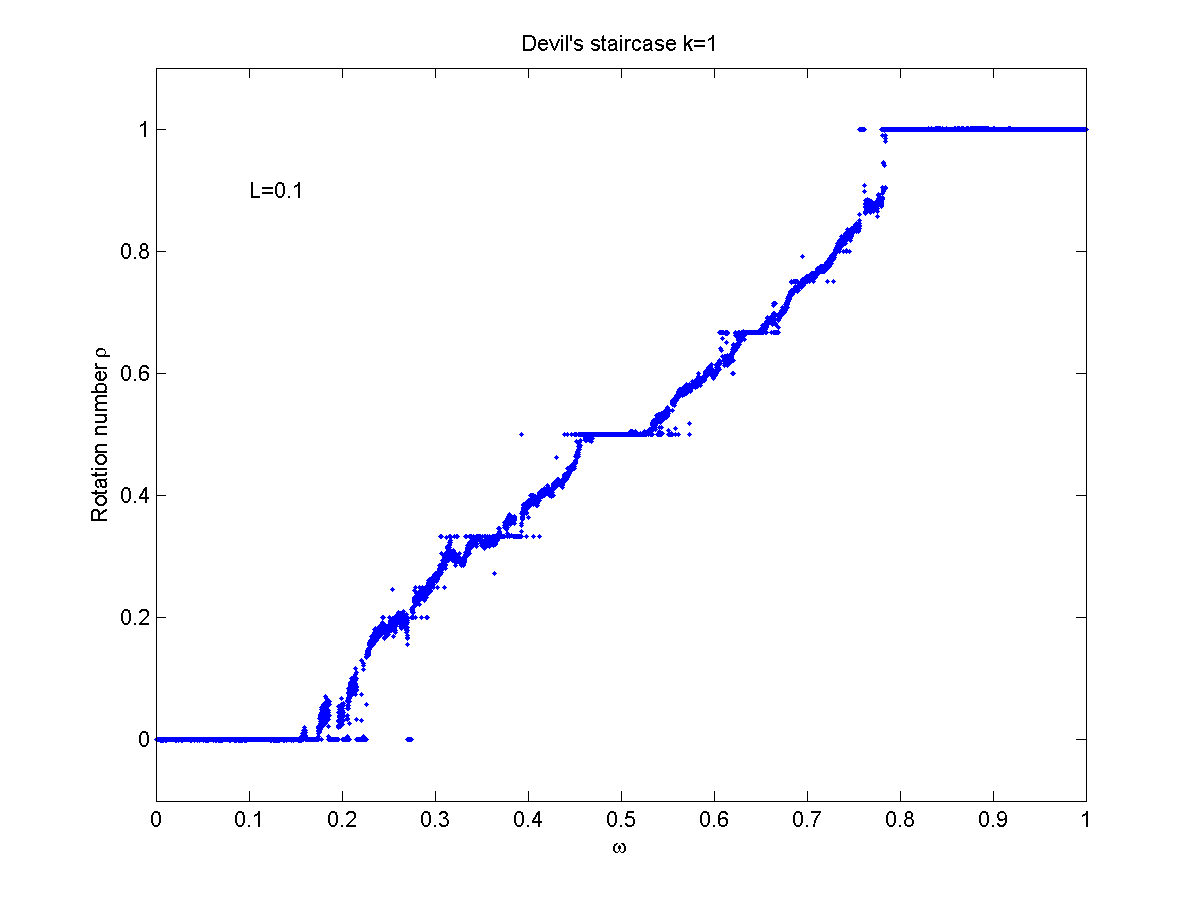
\includegraphics[width=.5\textwidth]{figs/rdevil_k1_L01.png}\hfill
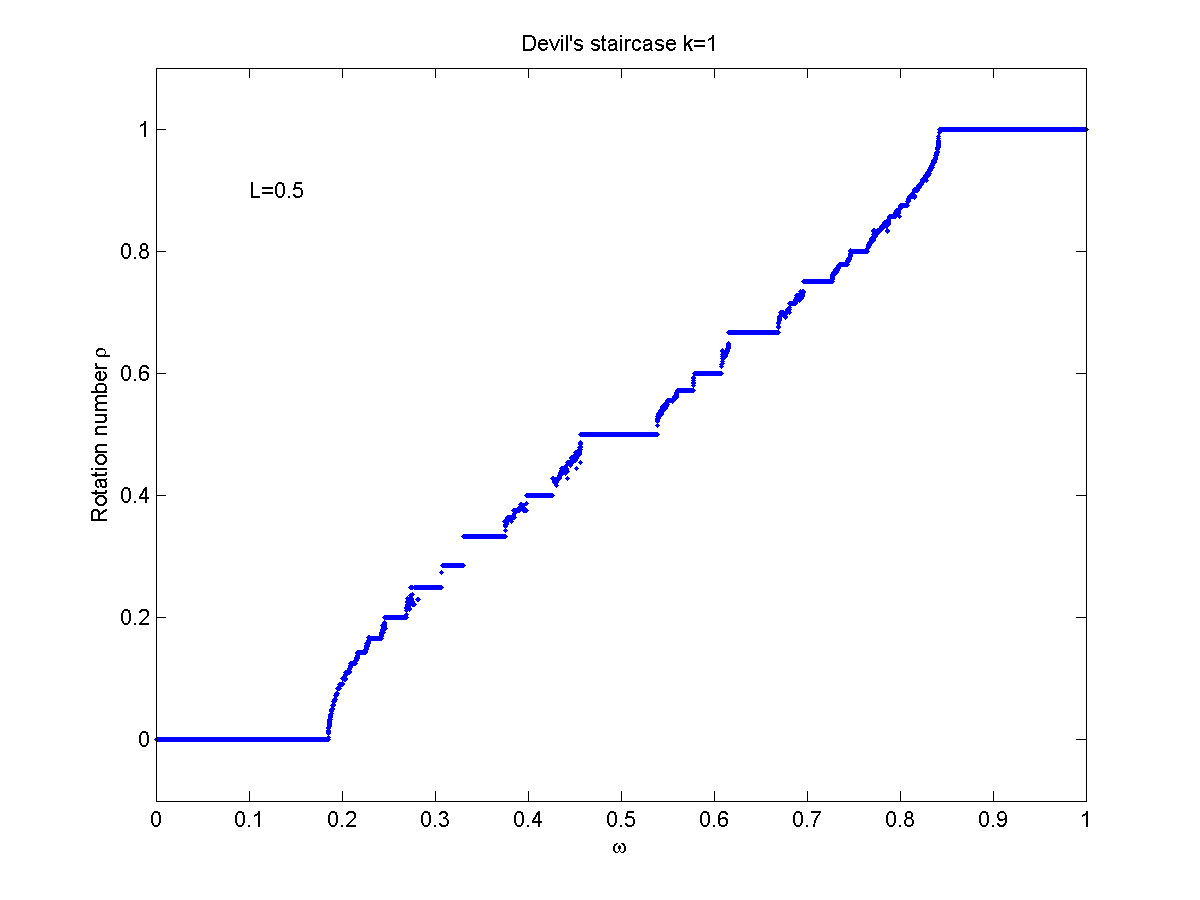
\includegraphics[width=.5\textwidth]{figs/rdevil_k1_L05.png}
\end{figure}

\begin{figure}[H]\linespread{1}
\caption[Histogram of rotation numbers in the random circle
map]{Histogram of rotation numbers in the random circle map, where
  $L=0.1$, $k=1$, $\alpha = 10^{-5}$,and $\omega = 0.45$. Results from 1000 simulations
  are plotted.}
\centering
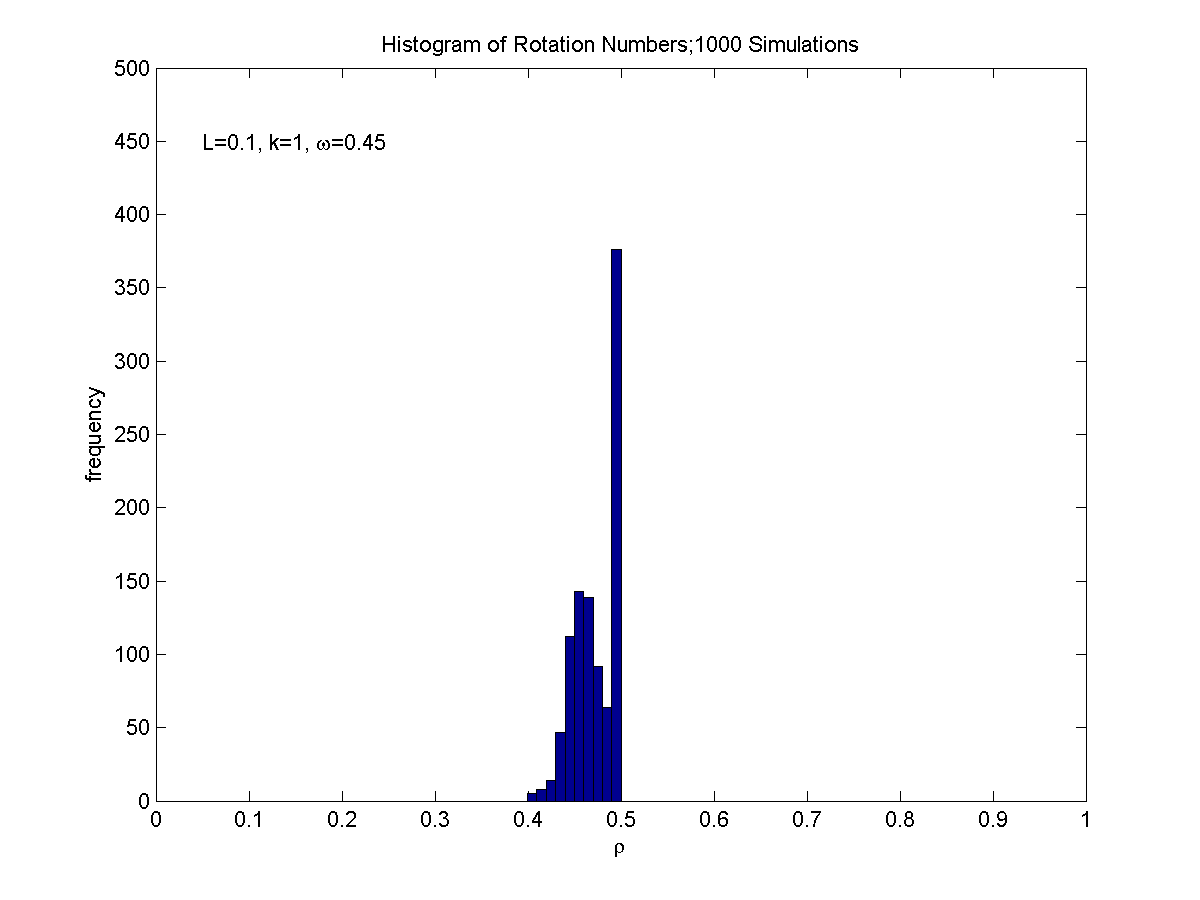
\includegraphics[width=.5\textwidth]{figs/hist_rho_k1_L01_om045.png}\hfill
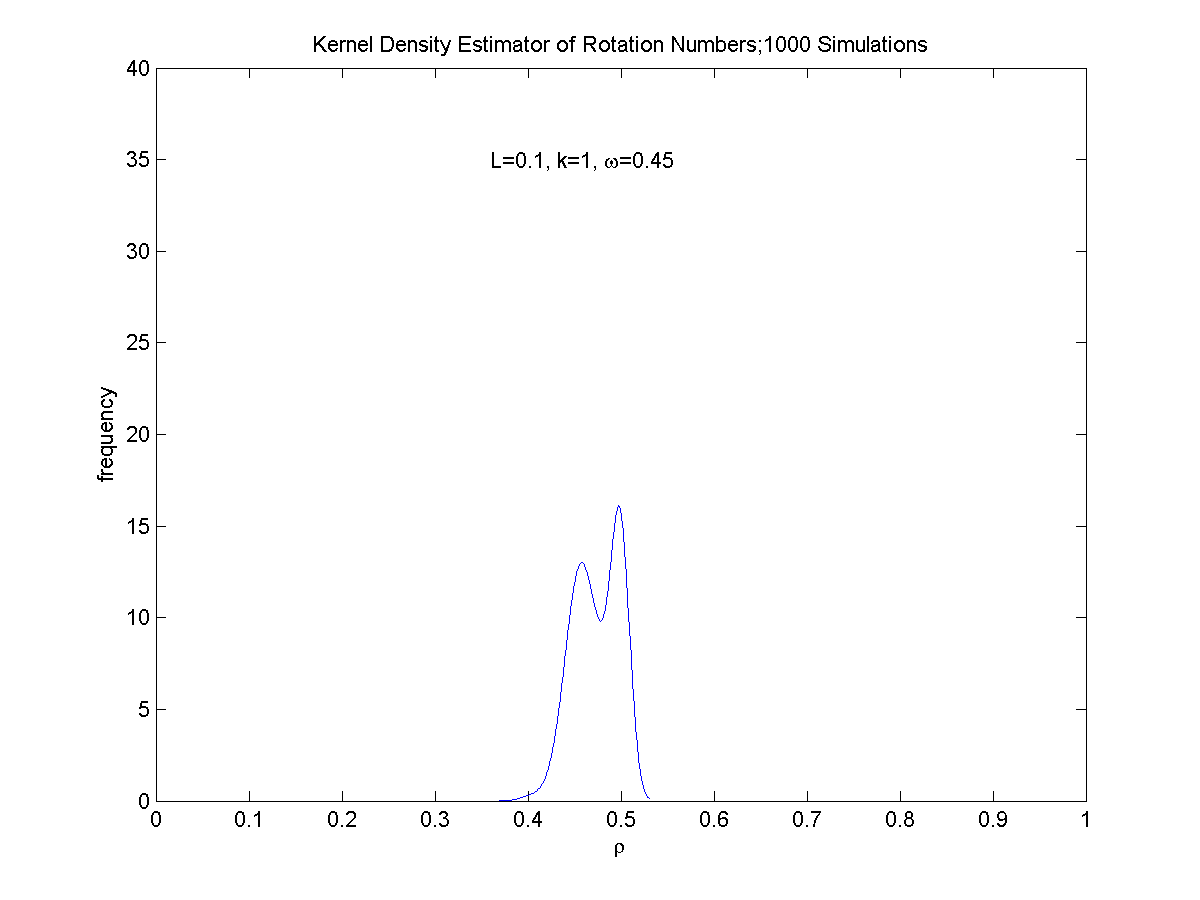
\includegraphics[width=.5\textwidth]{figs/kde_rho_k1_L01_om045.png}
\end{figure}

\begin{figure}[H]\linespread{1}  
\caption[The Arnold tongues for the random circle map, uniform distribution]{The Arnold
  tongues for $k\in [0,1.5]$, $\Delta k = 0.0015$, $\omega \in [0,1]$,
  $\Delta \omega = 0.001$, $\alpha = 10^{-5}$, $\hat{\xi}_n\sim Unif(-M_n,M_n)$ and $L_j \in
  \{10^{-6},0.05,0.1,0.3,0.5,0.9\}$. Plots are ordered left to right, and top to bottom. The colorbar
to the right demonstrates the period order and corresponding color.}\label{fig:randtongues}
\centering
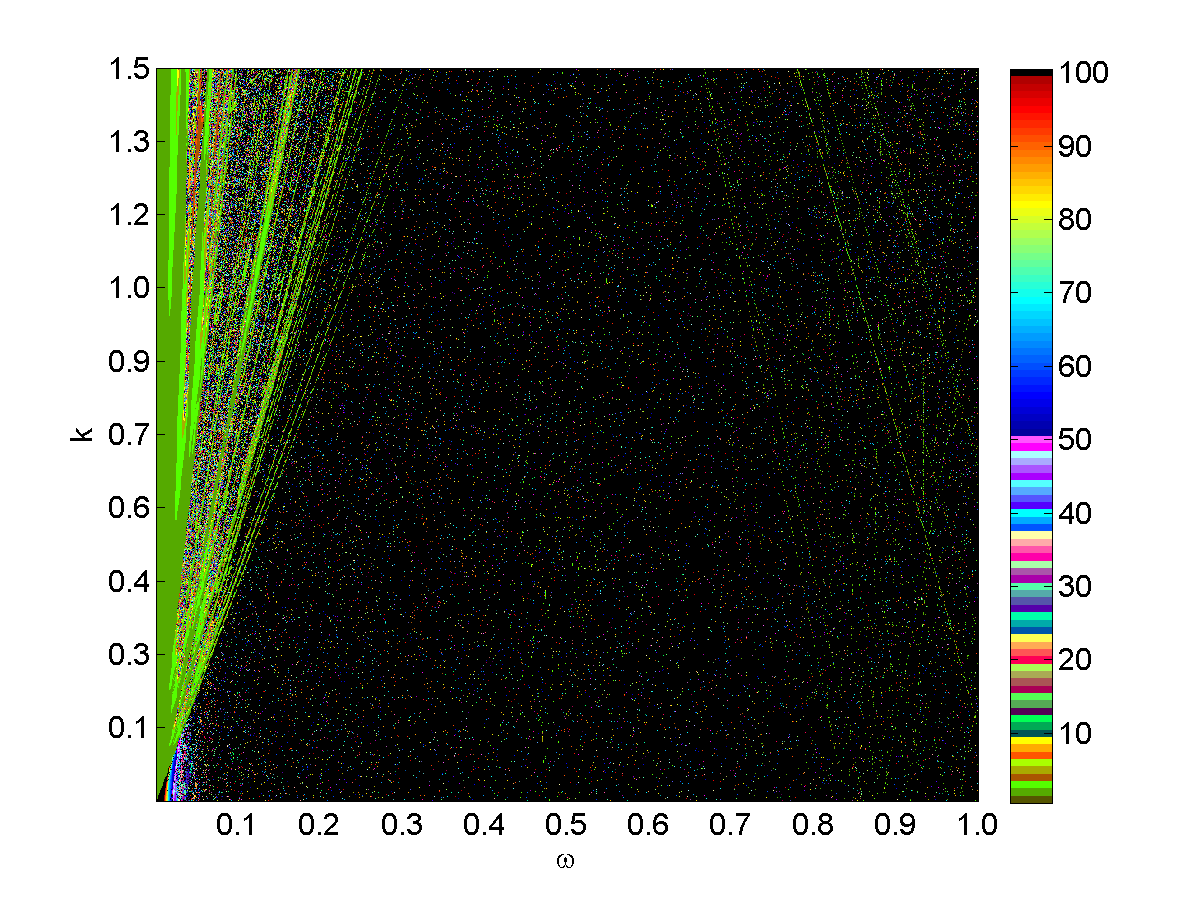
\includegraphics[width=.5\textwidth]{figs/tongues_1000_L_1e-05.png}\hfill
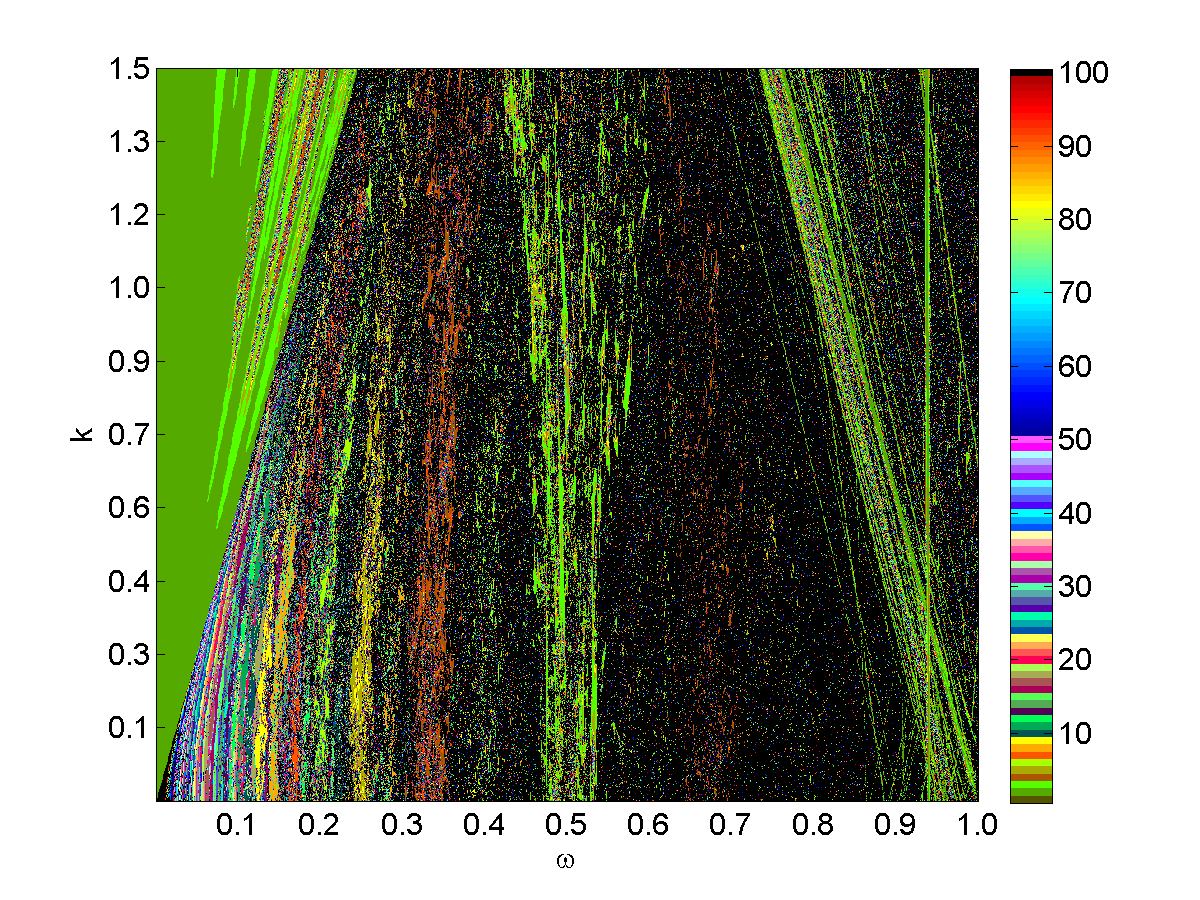
\includegraphics[width=.5\textwidth]{figs/tongues_1000_L_005.png}\\
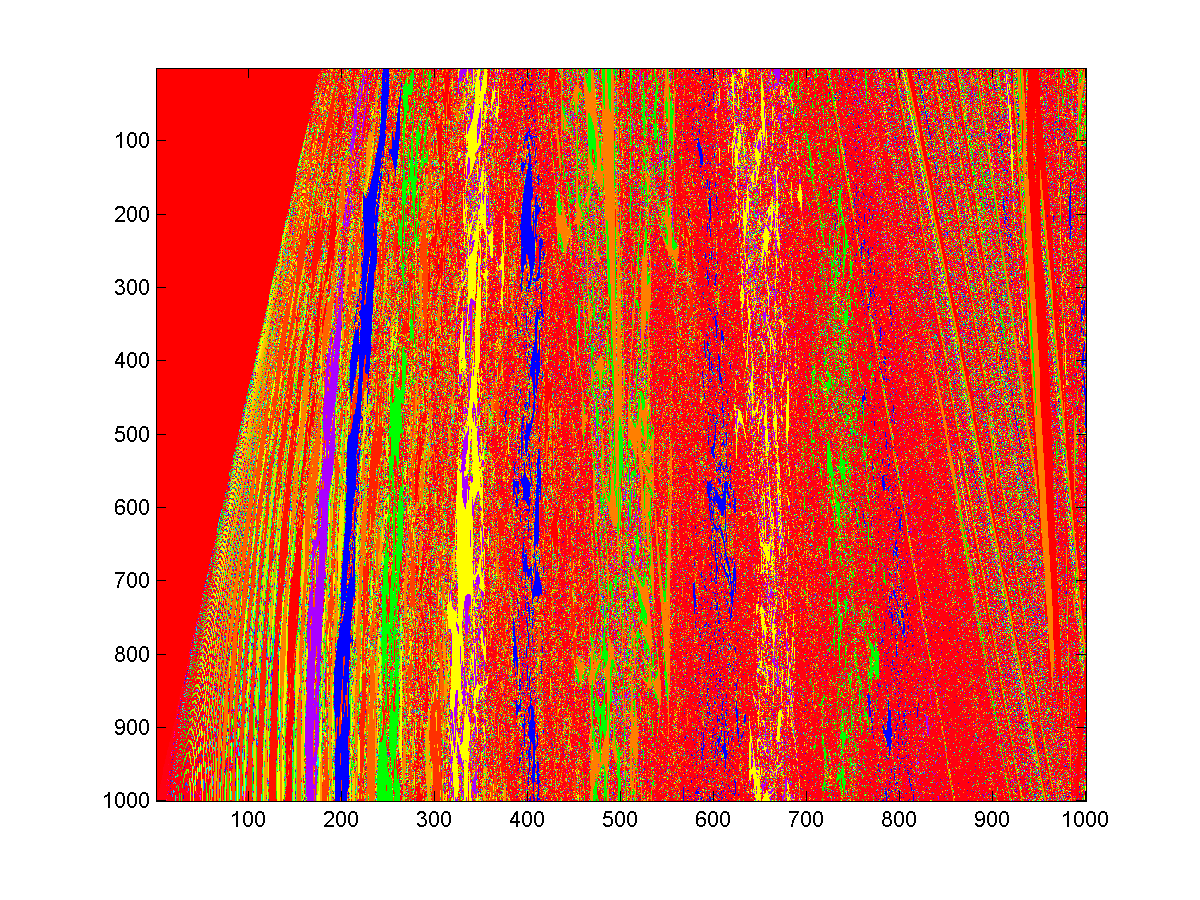
\includegraphics[width=.5\textwidth]{figs/tongues_1000_L_01.png}\hfill
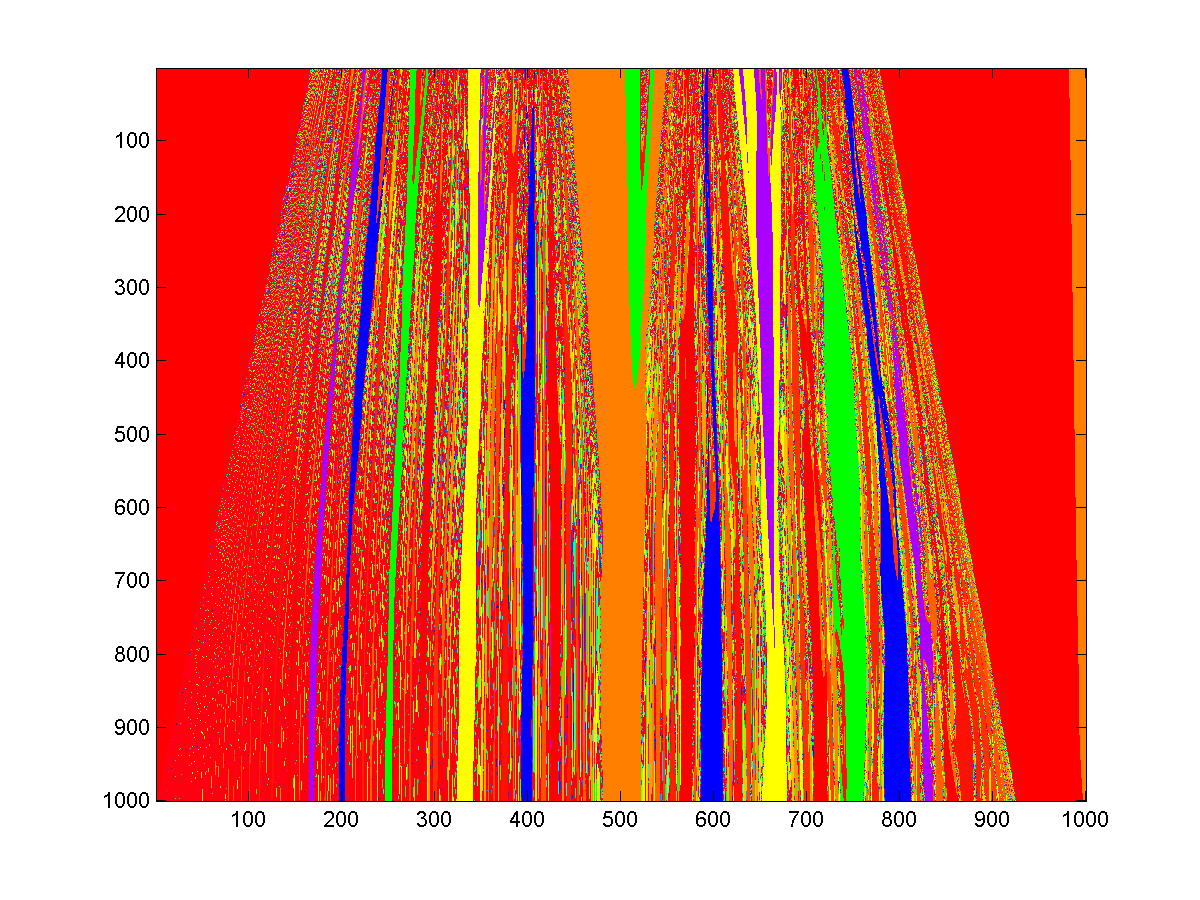
\includegraphics[width=.5\textwidth]{figs/tongues_1000_L_03.png}\\
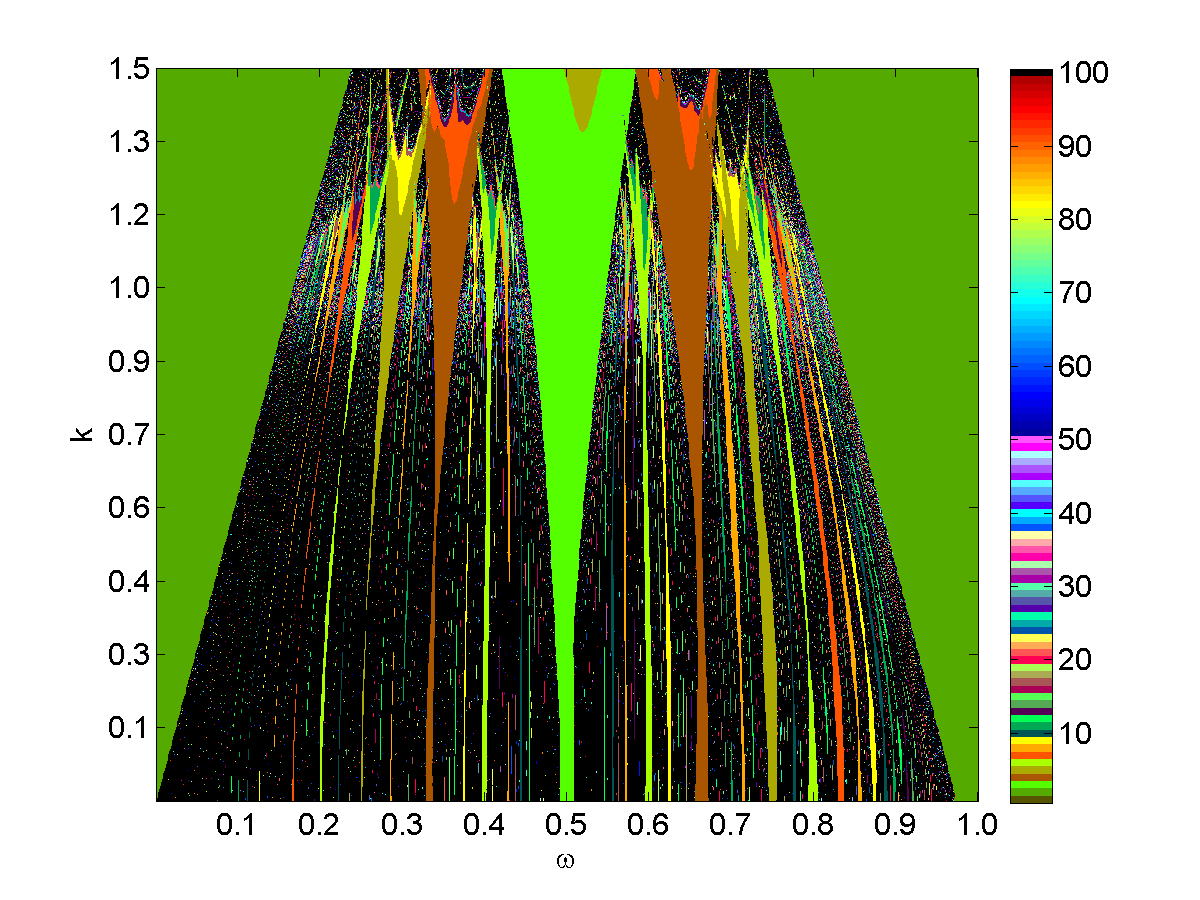
\includegraphics[width=.5\textwidth]{figs/tongues_1000_L_05.png}\hfill
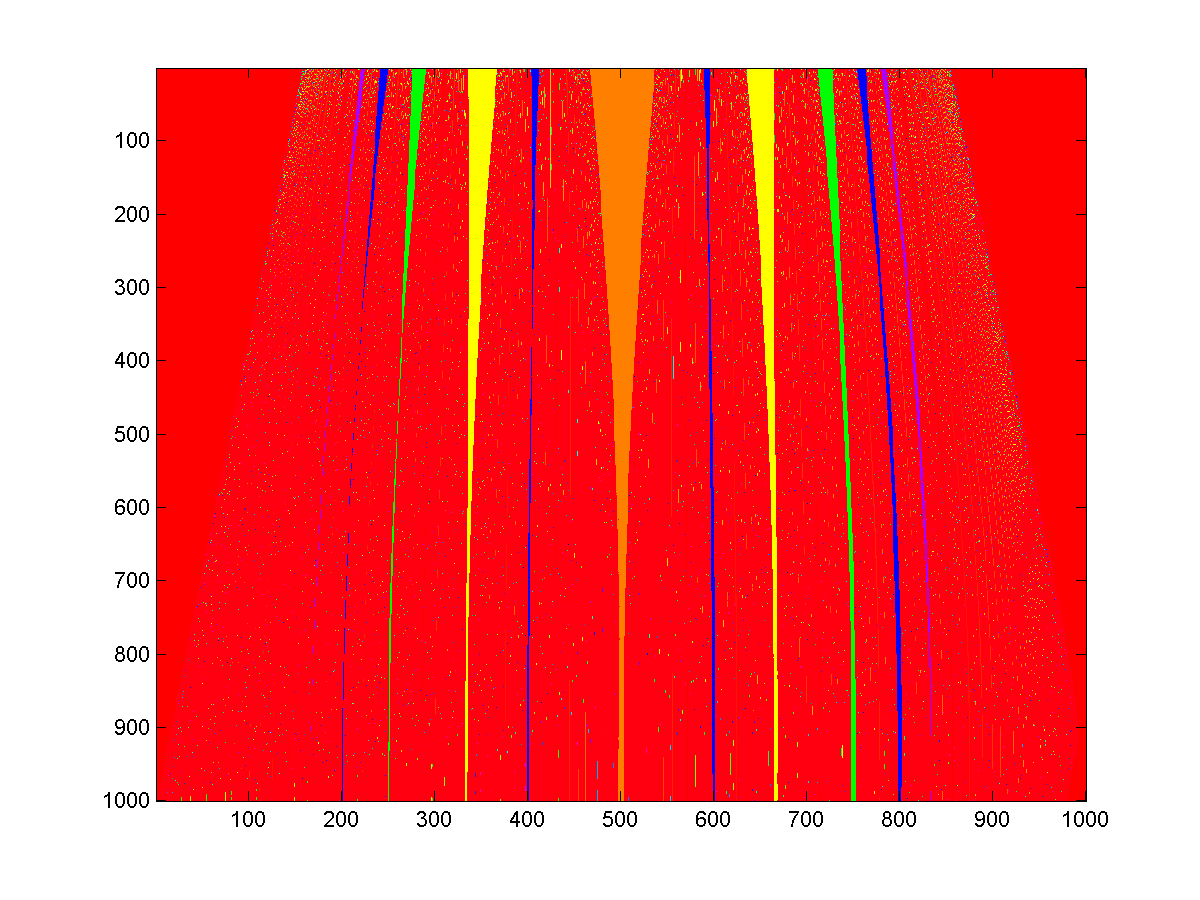
\includegraphics[width=.5\textwidth]{figs/tongues_1000_L_09.png}\\
\end{figure}
\subsection{Normal Distribution}
\begin{figure}[H]\linespread{1}  
\caption[The Arnold tongues for the random circle map, normal distribution]{The Arnold
  tongues for $k\in [0,1.5]$, $\Delta k = 0.0015$, $\omega \in [0,1]$,
  $\Delta \omega = 0.001$, $\alpha = 10^{-5}$, $\hat{\xi}_n\sim
  N(0,\alpha e^{-L|n|})$ and $L_j \in
  \{0.025,0.05,0.1,0.3,0.5,0.9\}$. Plots are ordered left to right, and top to bottom. The colorbar
to the right demonstrates the period order and corresponding color.}\label{fig:randtongues}
\centering
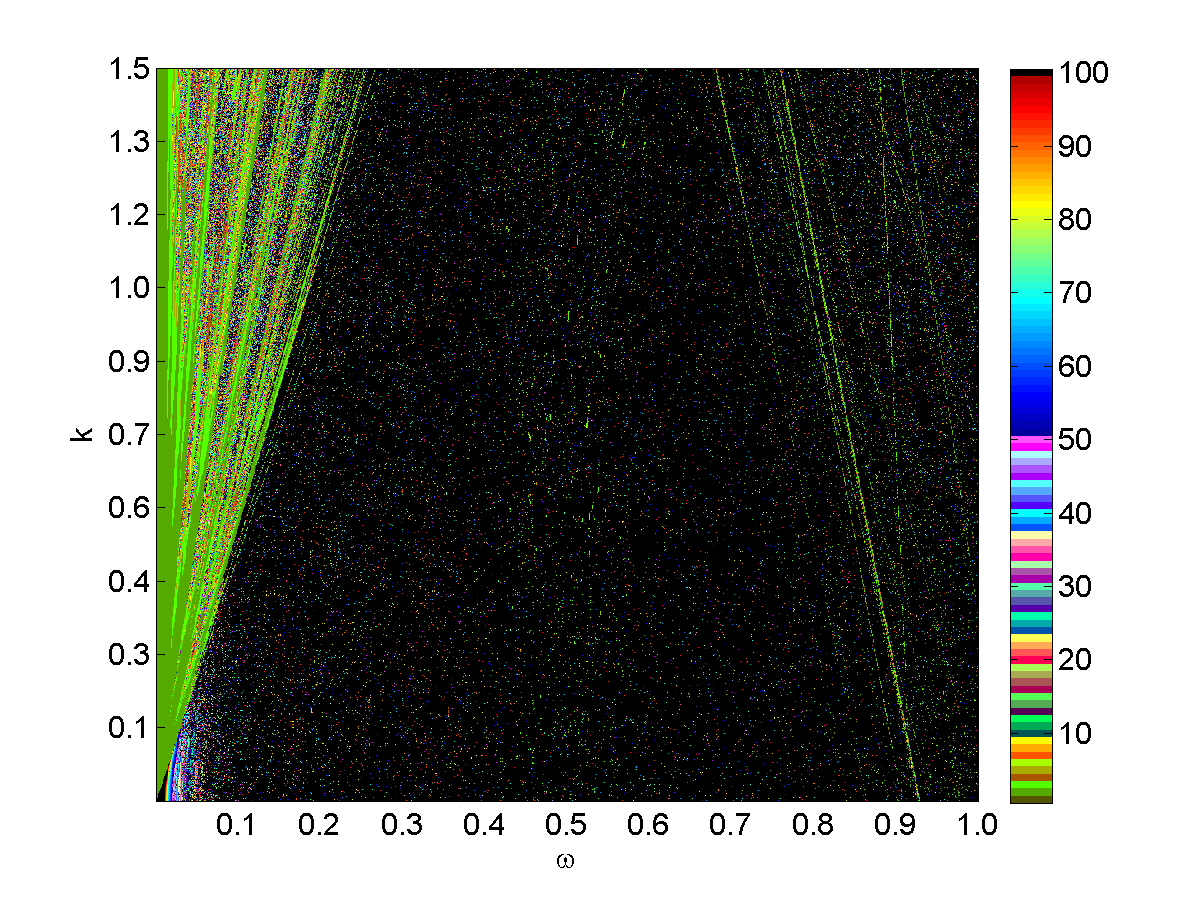
\includegraphics[width=.5\textwidth]{figs/tongues_norm_1000_L_0025.png}\hfill
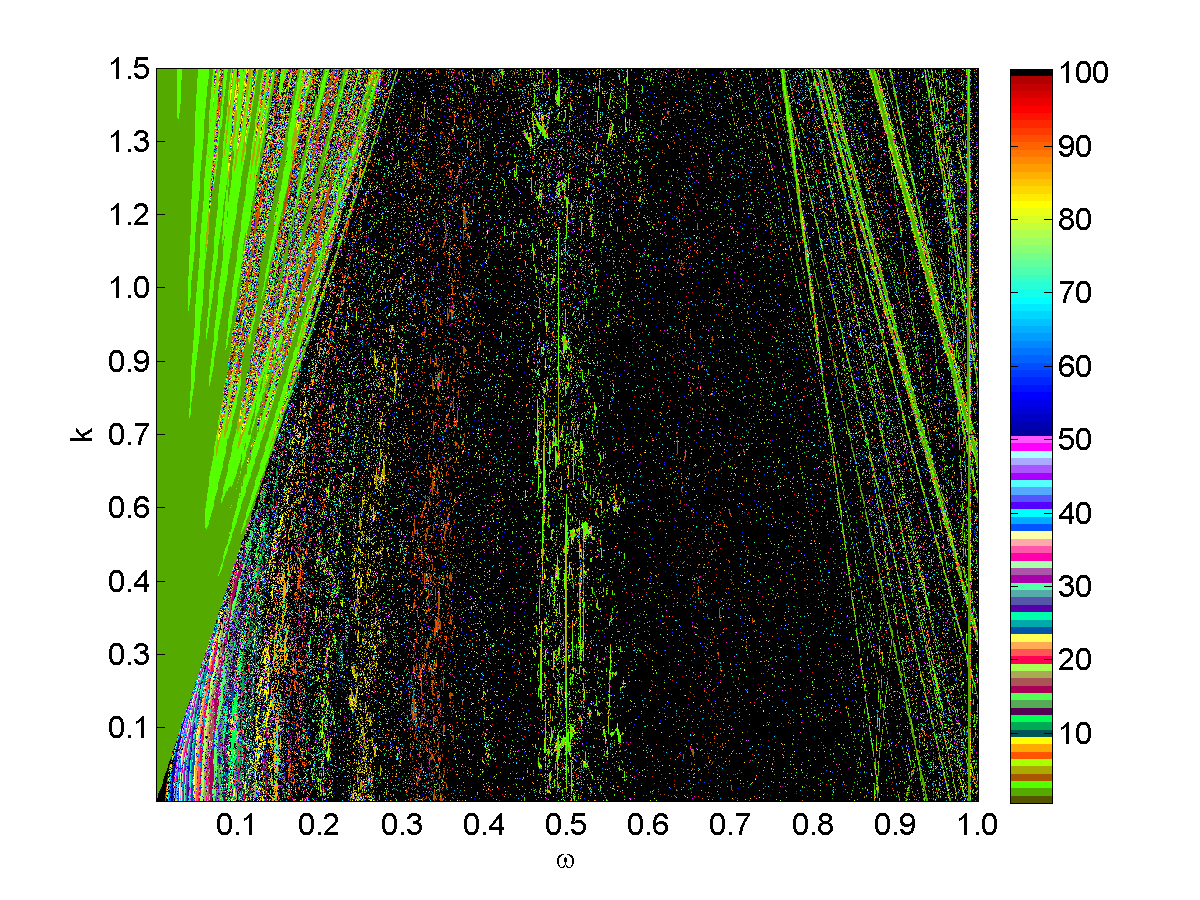
\includegraphics[width=.5\textwidth]{figs/tongues_norm_1000_L_005.png}\\
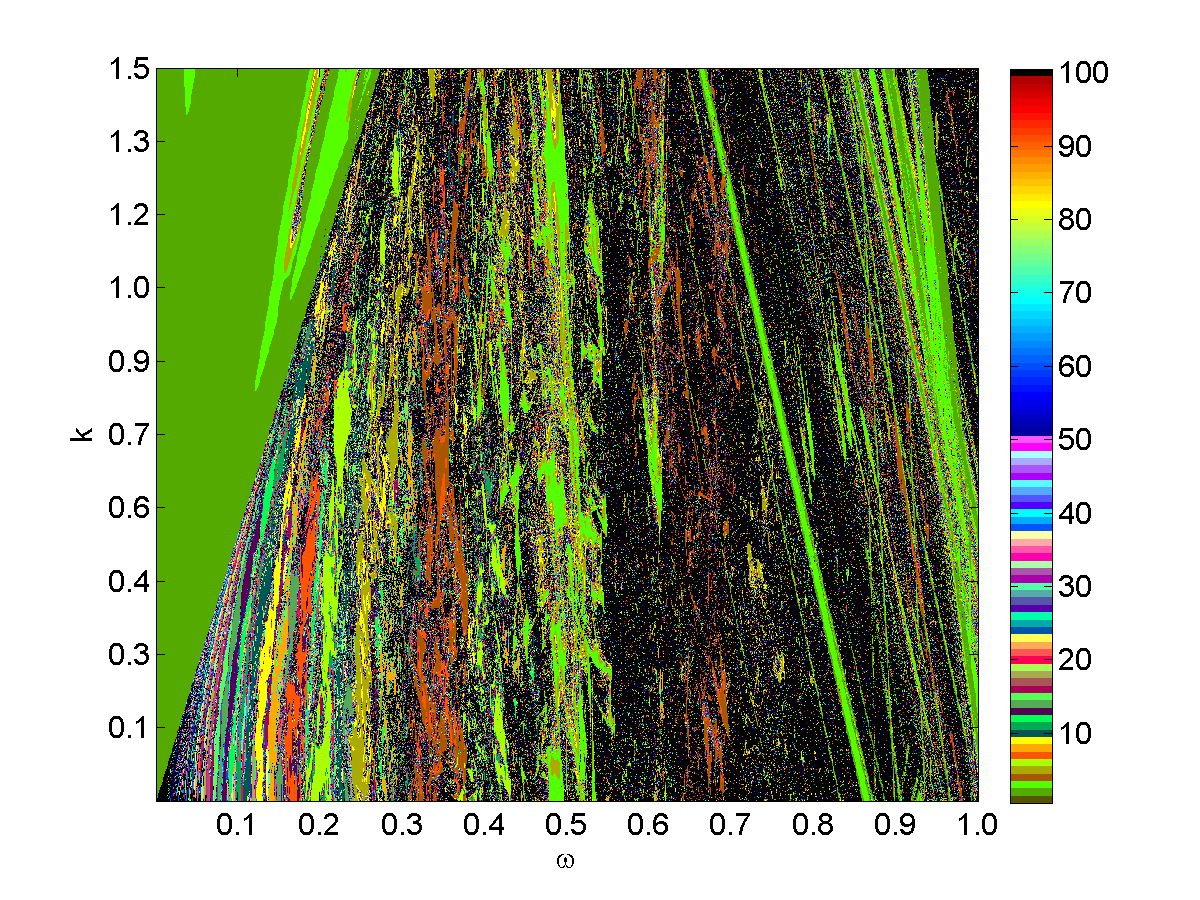
\includegraphics[width=.5\textwidth]{figs/tongues_norm_1000_L_01.png}\hfill
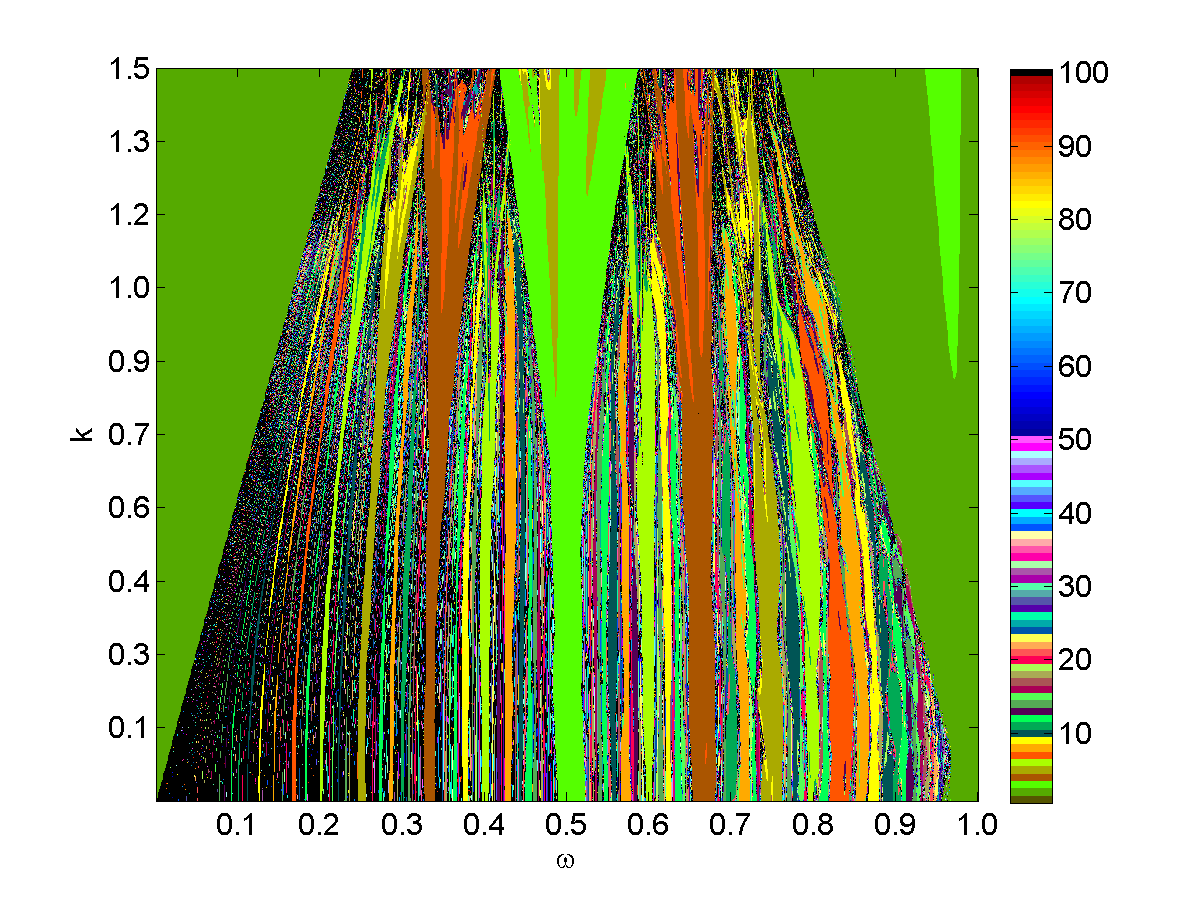
\includegraphics[width=.5\textwidth]{figs/tongues_norm_1000_L_03.png}\\
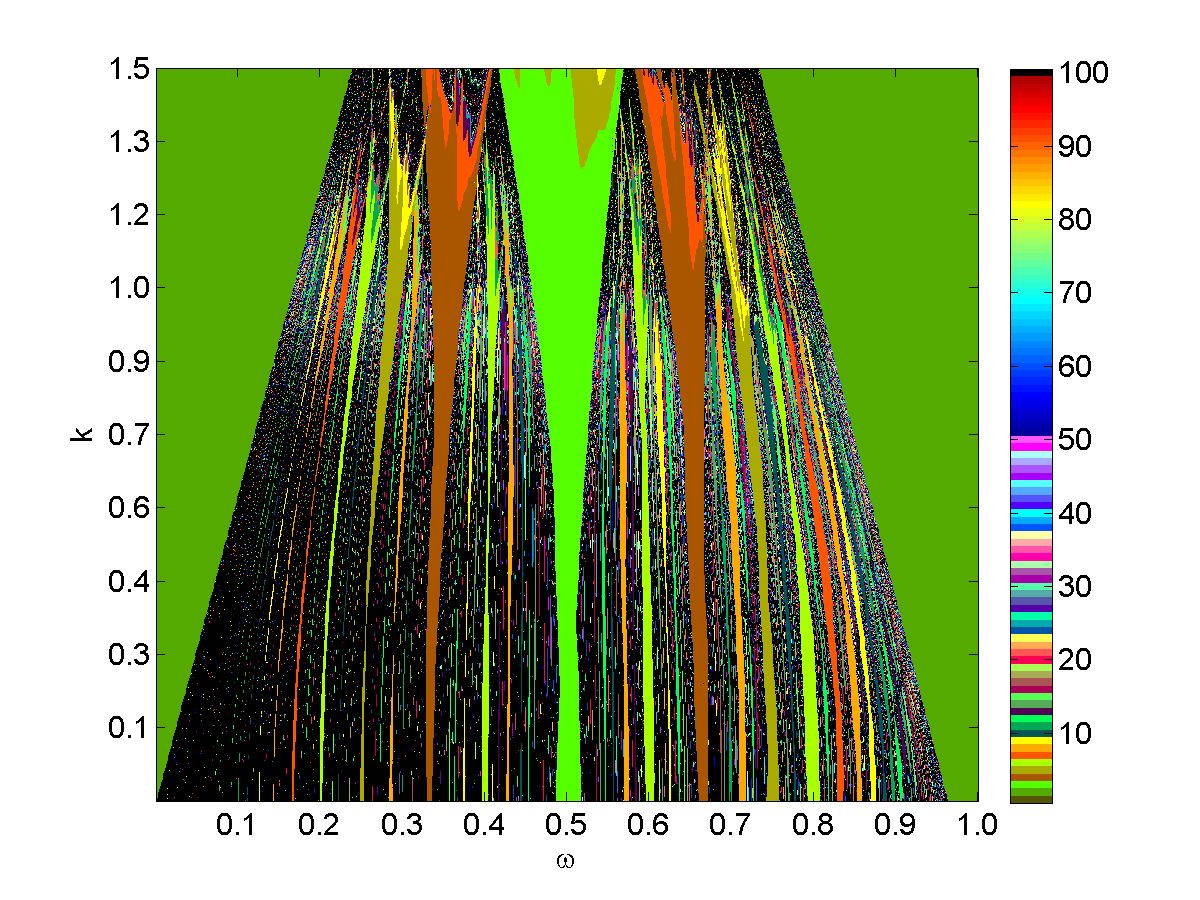
\includegraphics[width=.5\textwidth]{figs/tongues_norm_1000_L_05.png}\hfill
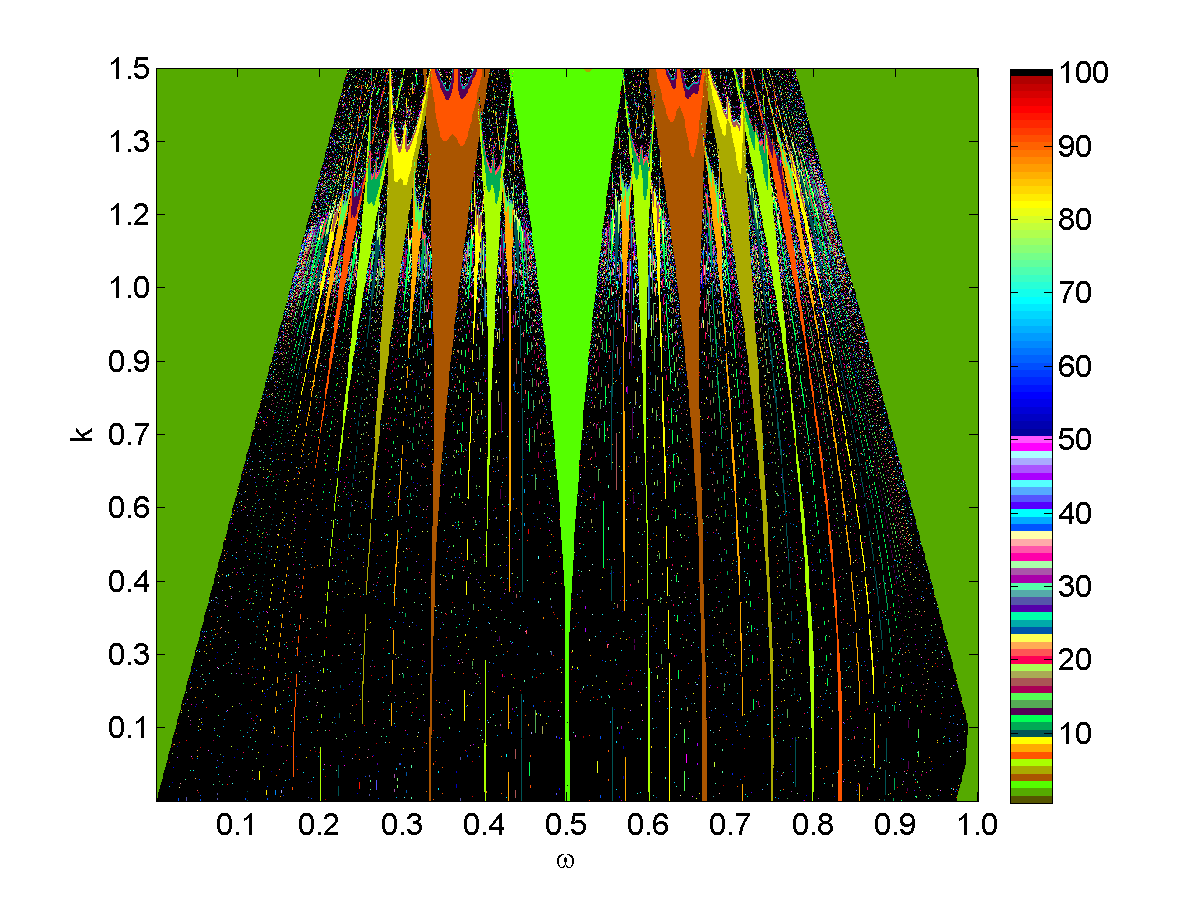
\includegraphics[width=.5\textwidth]{figs/tongues_norm_1000_L_09.png}\\
\end{figure}

\begin{figure}[!h]
\caption[Lyapunov exponent in the random circle map (normal distribution) compared to the
deterministic map, varying $\omega$]{The Lyapunov exponent for the deterministic
  circle map (top left) is compared
  to the Lyapunov exponent of the random circle map for $L \in
  \{0.05,0.1,0.3,0.5,0.9\}$, where $x_0=0.7$, $k=1.5$,$\alpha =
  10^{-5}$, and $\hat{\xi}_n\sim
  N(0,\alpha e^{-L|n|})$ for $\omega \in [0,1]$. The number of exponents computed was $N_\lambda=10,000$. Plots are read left to right, and top to bottom. }\label{fig:rloglyap2}
\centering
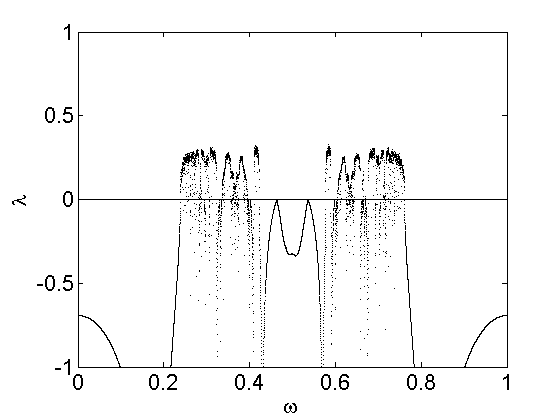
\includegraphics[width=.5\textwidth]{figs/det_circ_lyap.png}\hfill
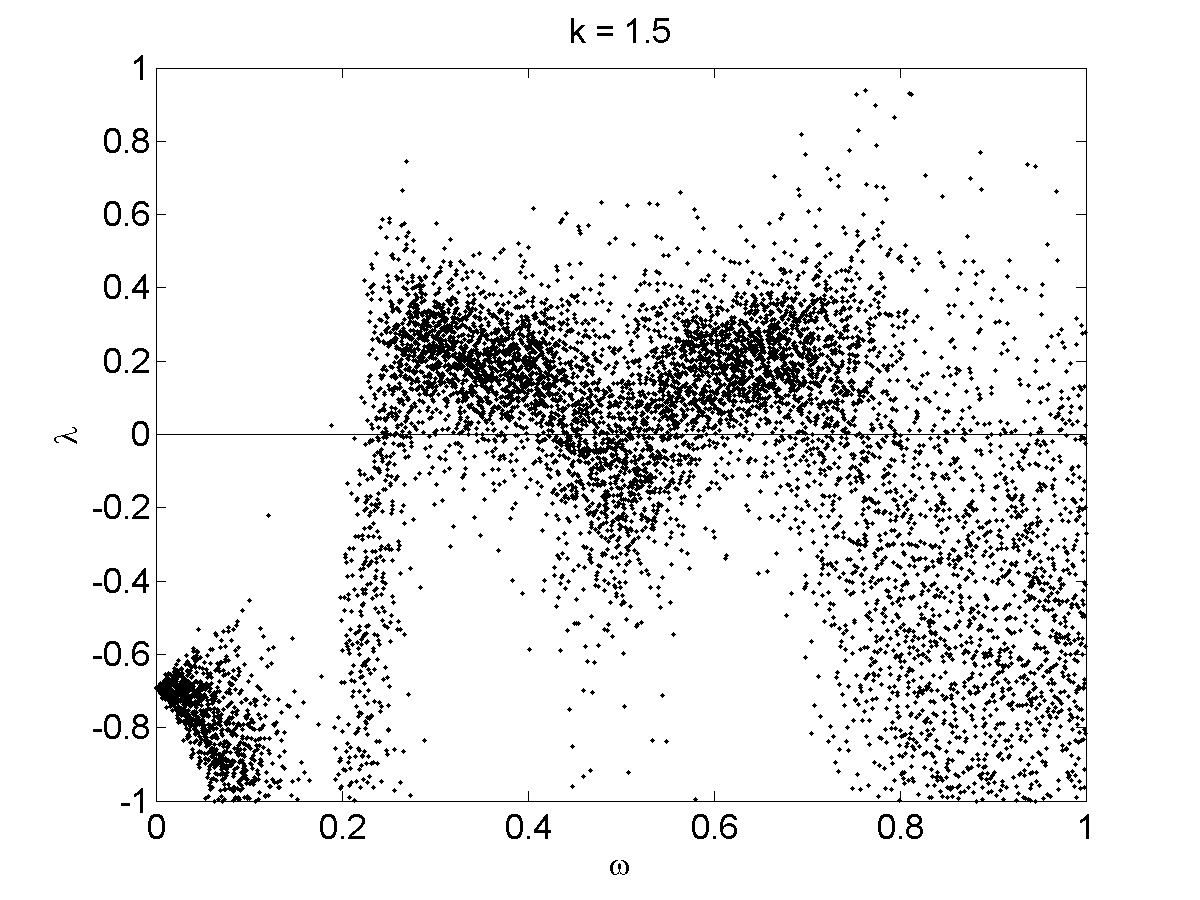
\includegraphics[width=.5\textwidth]{figs/rcirc_n_lyap_L_005_w.png}\\
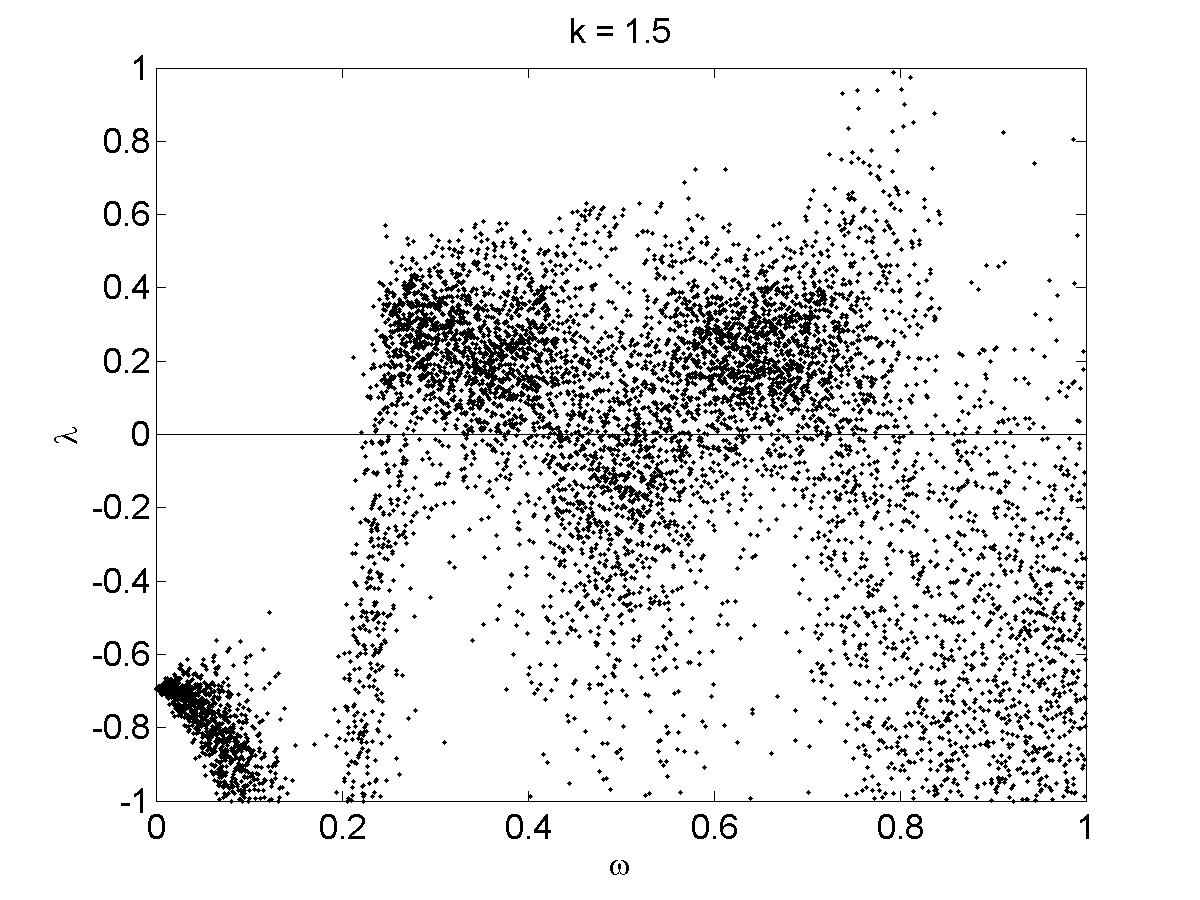
\includegraphics[width=.5\textwidth]{figs/rcirc_n_lyap_L_01_w.png}\hfill
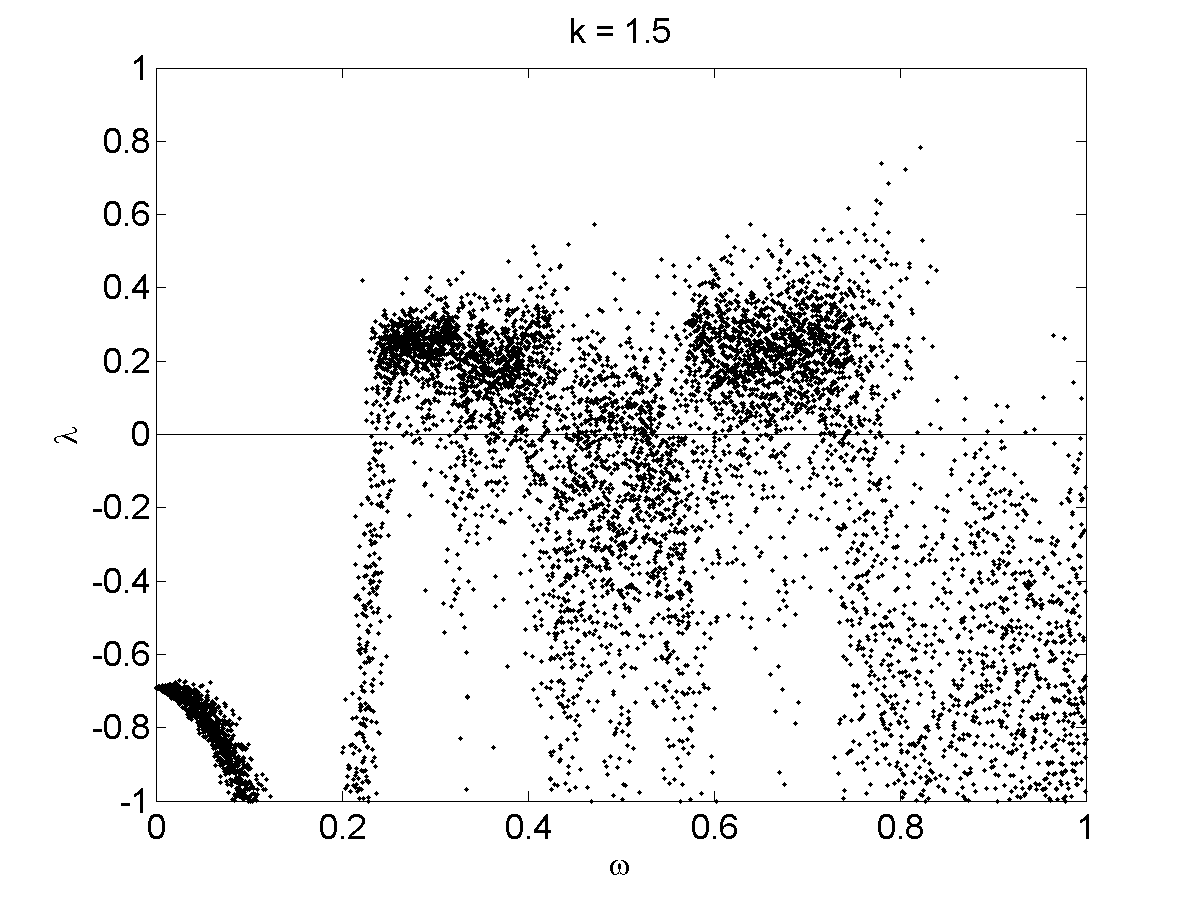
\includegraphics[width=.5\textwidth]{figs/rcirc_n_lyap_L_03_w.png}\\
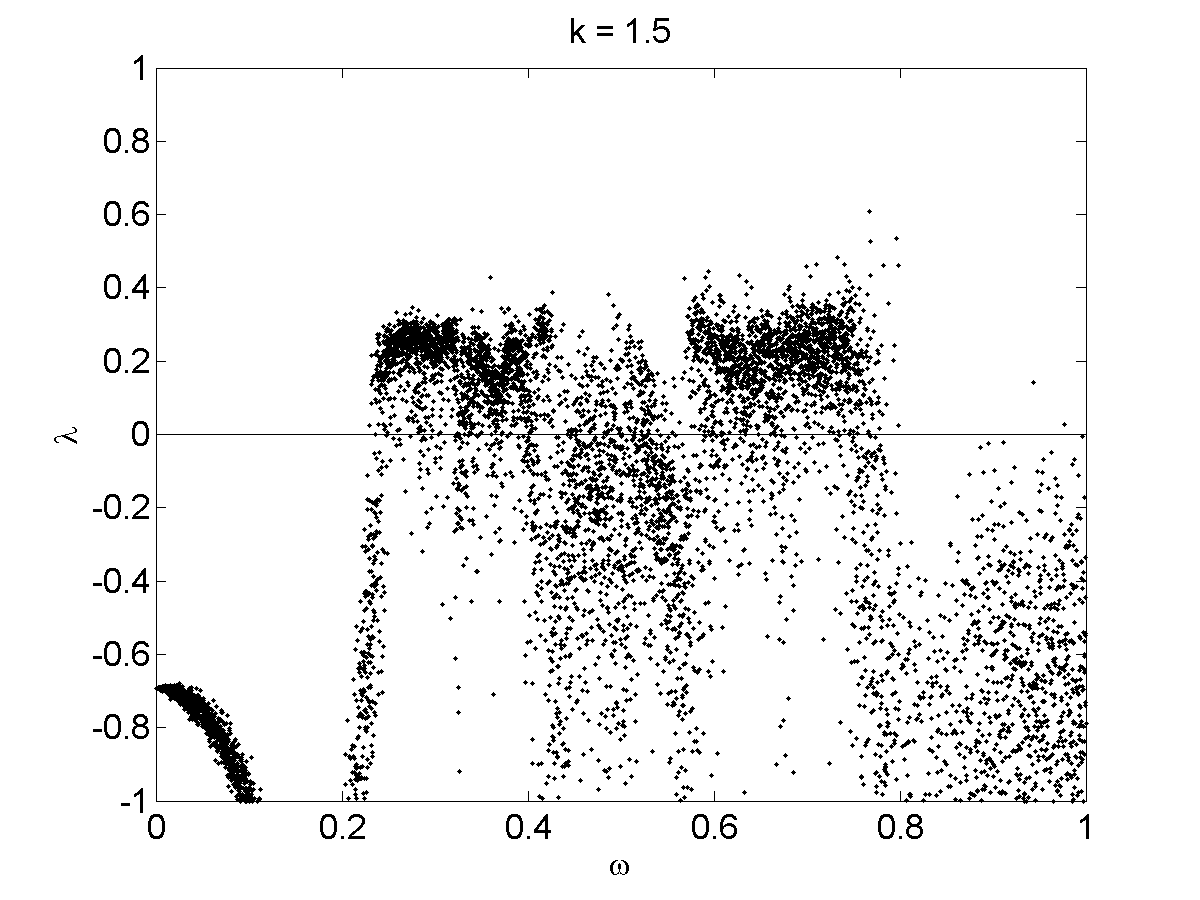
\includegraphics[width=.5\textwidth]{figs/rcirc_n_lyap_L_05_w.png}\hfill
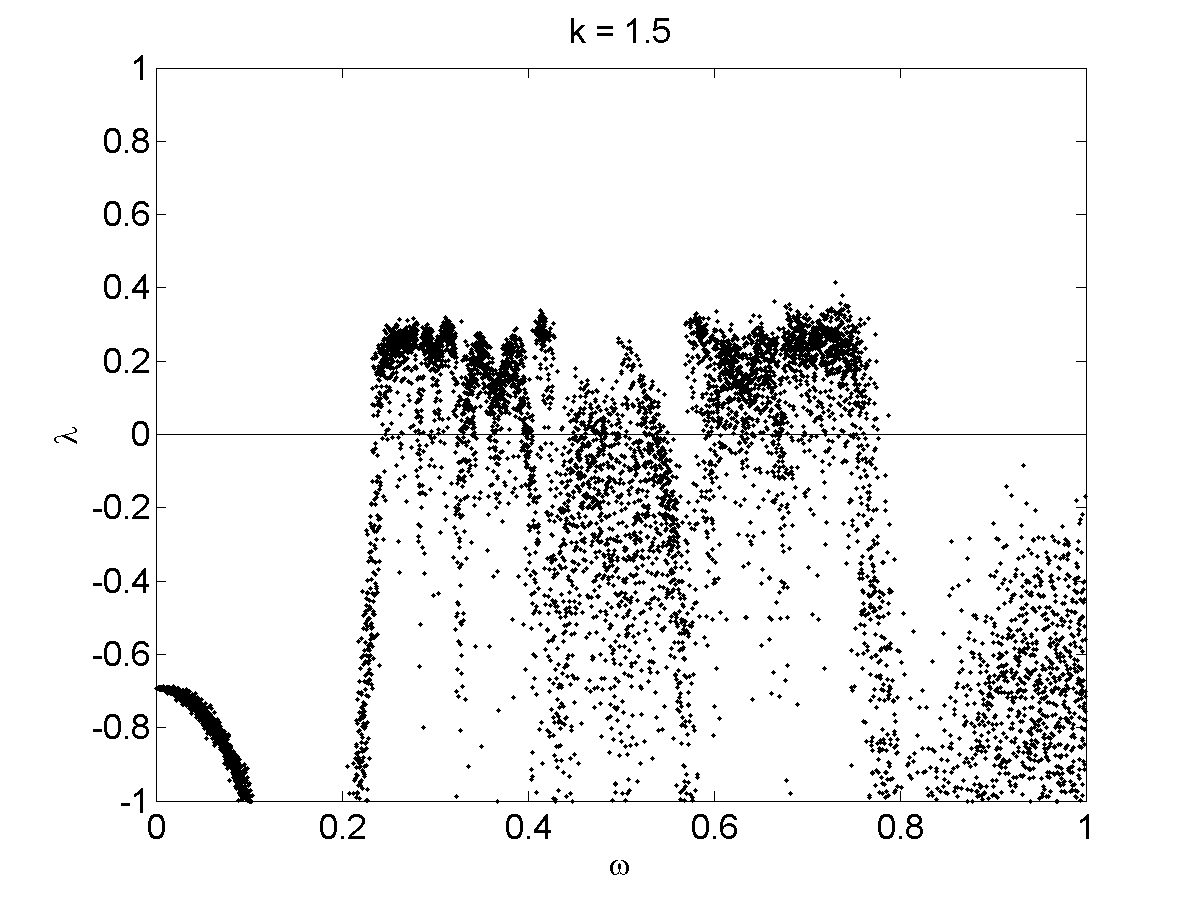
\includegraphics[width=.5\textwidth]{figs/rcirc_n_lyap_L_09_w.png}\\
\end{figure}

\begin{figure}[!h]
\caption[Lyapunov exponent in the random circle map (normal distribution) compared to the
deterministic map, varying $k$]{The Lyapunov exponent for the deterministic
  circle map (top left) is compared
  to the Lyapunov exponent of the random circle map for $L \in
  \{0.05,0.1,0.3,0.5,0.7\}$, where $x_0=0.7$, $\omega=0.7$,$\alpha =
  10^{-5}$, and $\hat{\xi}_n\sim
  N(0,\alpha e^{-L|n|})$ for $k \in [0,5]$. The number of exponents computed was $N_\lambda=10,000$. Plots are read left to right, and top to bottom. }\label{fig:rloglyap2}
\centering
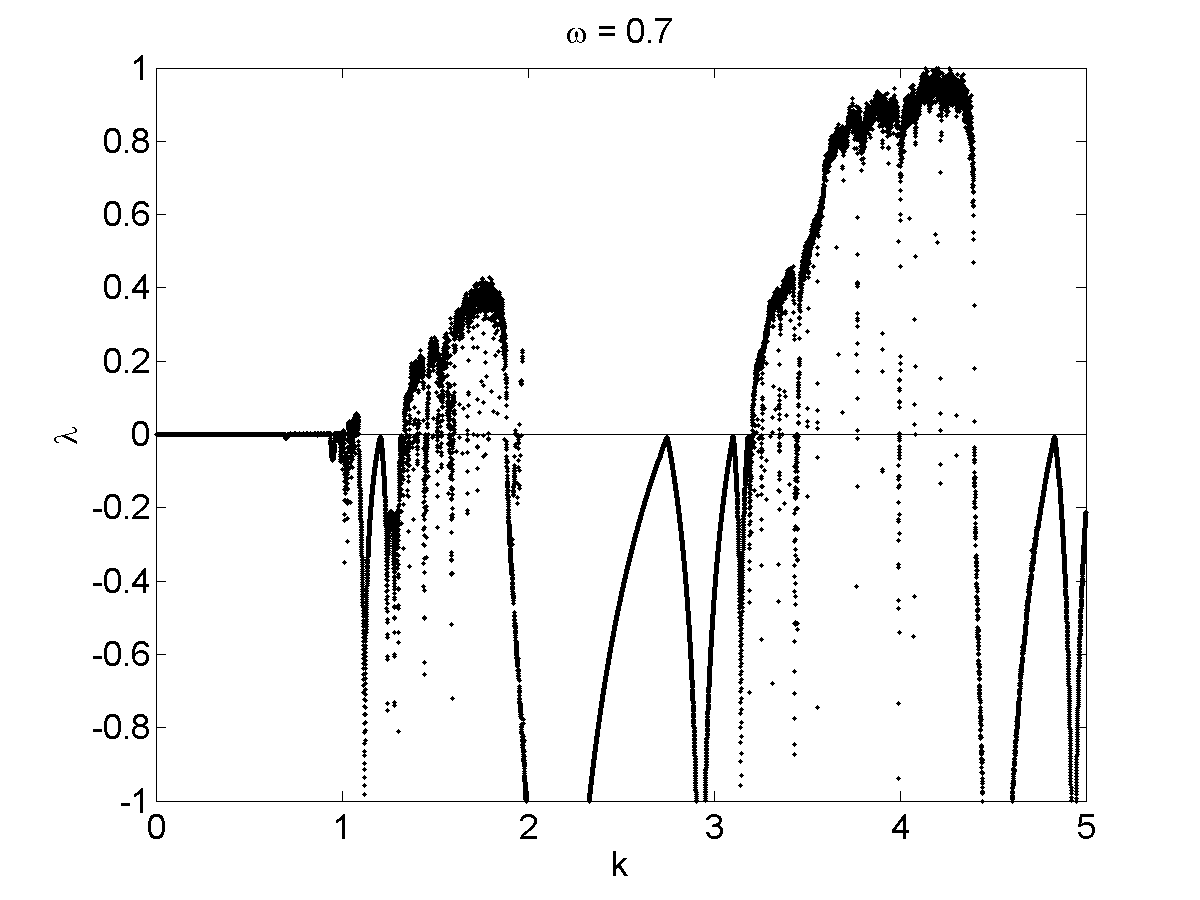
\includegraphics[width=.5\textwidth]{figs/det_circ_lyap_k.png}\hfill
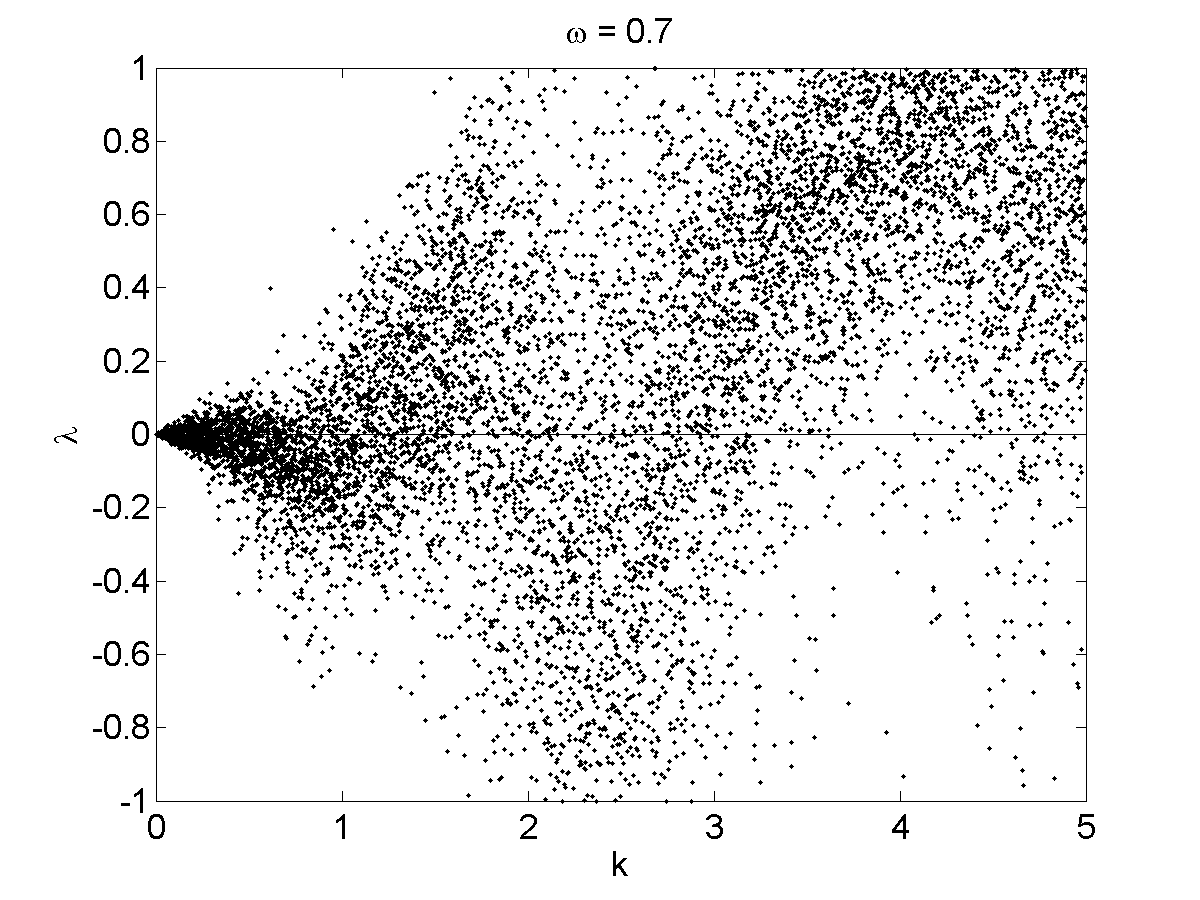
\includegraphics[width=.5\textwidth]{figs/rcirc_n_lyap_L_005_k_10000.png}\\
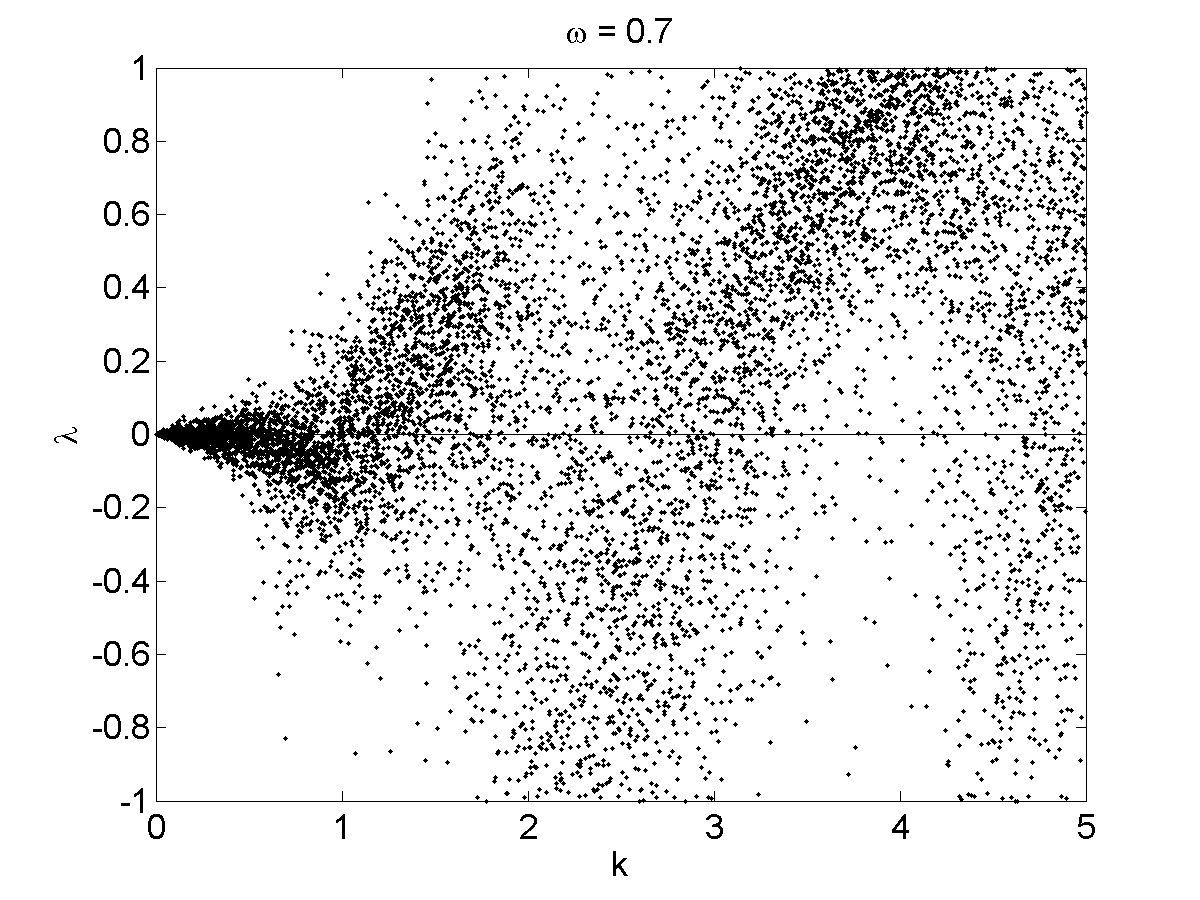
\includegraphics[width=.5\textwidth]{figs/rcirc_n_lyap_L_01_k_10000.png}\hfill
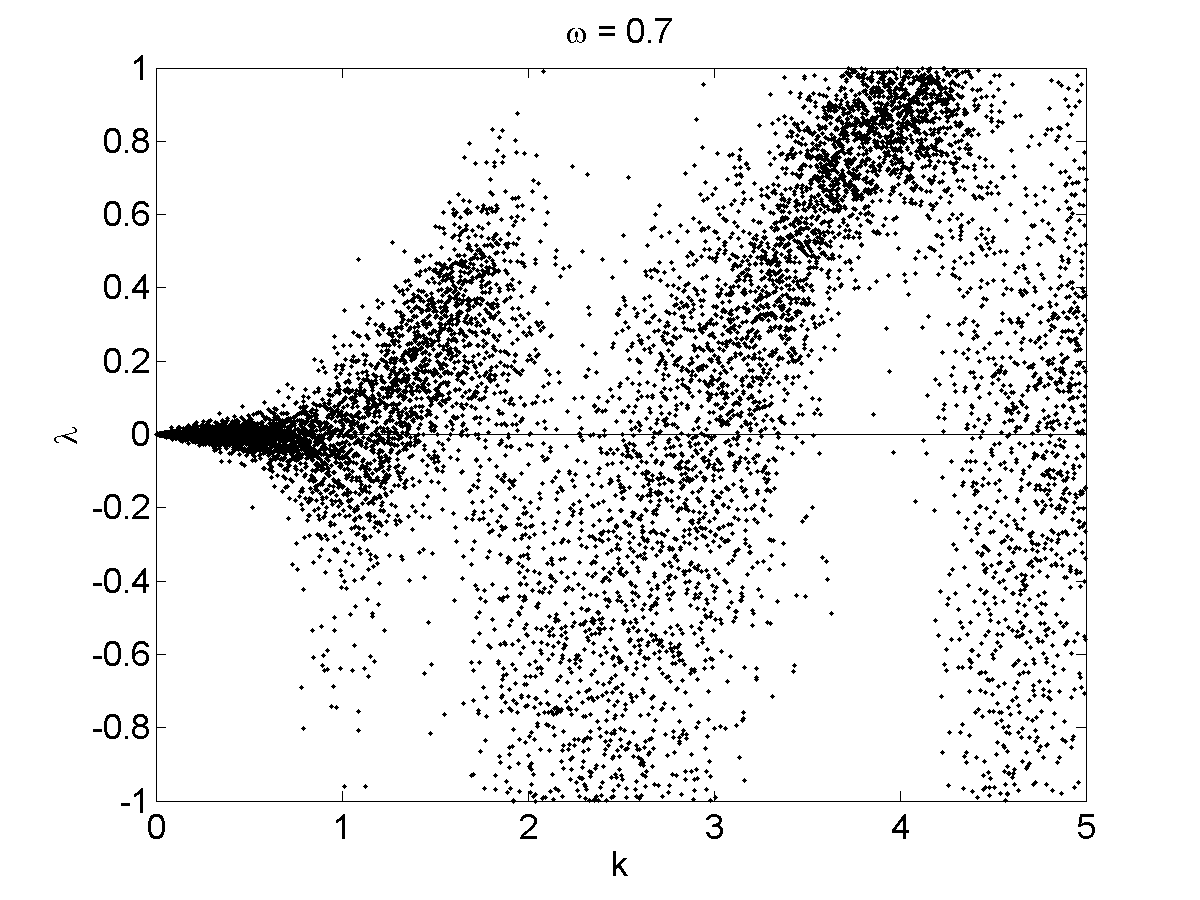
\includegraphics[width=.5\textwidth]{figs/rcirc_n_lyap_L_03_k_10000.png}\\
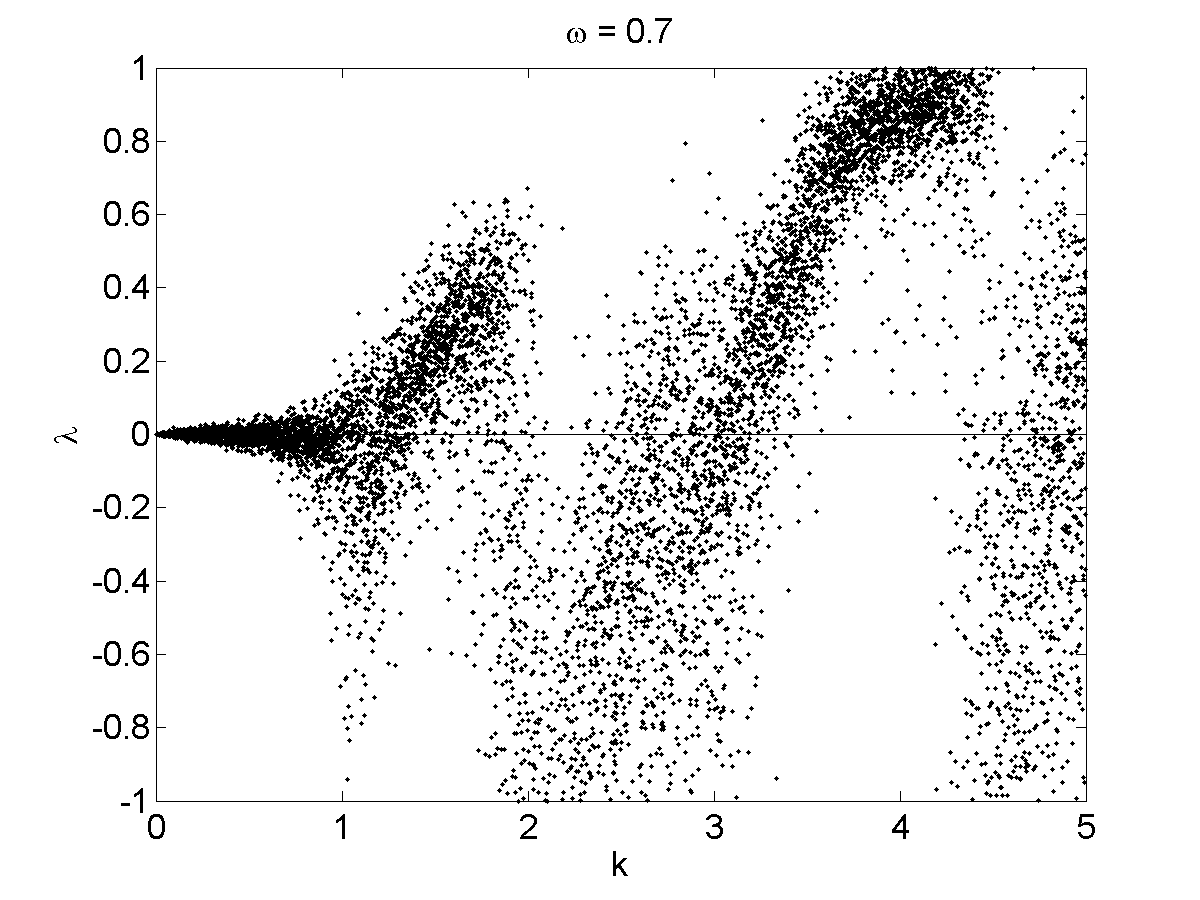
\includegraphics[width=.5\textwidth]{figs/rcirc_n_lyap_L_05_k_10000.png}\hfill
\includegraphics[width=.5\textwidth]{figs/rcirc_n_lyap_L_07_k_10000.png}\\
\end{figure}